\documentclass[11pt]{book}

\usepackage{epsfig}
\usepackage{html}
\usepackage{hypre}
\usepackage{makeidx}
\usepackage{graphicx}

%=============================================================================
% Preamble:
%=============================================================================

% set margins
\setlength{\oddsidemargin}{0in}
\setlength{\evensidemargin}{0in}
\setlength{\textwidth}{6.5in}
\setlength{\topmargin}{0in}
\setlength{\textheight}{8.0in}

% define various commands and macros

% define the version number
% NOTE: this is automatically generated from another file in hypre
\def\HYPREVersion{2.4.0b}
\def\HYPREVersionDate{2008/08/08}


% write out the index entries in the `.idx' file
\makeindex

%=============================================================================
% Body:
%=============================================================================

\begin{document}

%=============== Title Page

\begin{TitlePage}

\Title{User's Manual}
\SubTitle{Software Version: \HYPREVersion}
\SubTitle{Date: \HYPREVersionDate}
\vfill
\begin{center}
\InsertGraphics{hypre_wiw}{width=.7\textwidth}
\end{center}
\vfill
\Author{%
Center for Applied Scientific Computing\\
Lawrence Livermore National Laboratory
}

\end{TitlePage}

%=============== Copyright Page

\begin{CopyrightPage}
\noindent
Copyright (c) 2006   The Regents of the University of California.
Produced at the Lawrence Livermore National Laboratory.
Written by the HYPRE team, (hypre-users@llnl.gov), UCRL-CODE-222953.
All rights reserved.

\vspace{1em}\noindent
This notice is required to be provided under our contract with the U.S. 
Department of Energy (DOE). This work was produced at the University of 
California, Lawrence Livermore National Laboratory under Contract No. W7405-ENG-48 with the DOE.
 
\vspace{1em}\noindent
Neither the United States Government nor the University of California nor any 
of their employees, makes any warranty, express or implied, or assumes any 
liability or responsibility for the accuracy, completeness, or usefulness of any 
information, apparatus, product, or process disclosed, or represents that its use 
would not infringe privately-owned rights. 

\vspace{1em}\noindent
Also, reference herein to any specific commercial products, process, or 
services by trade name, trademark, manufacturer or otherwise does not 
necessarily constitute or imply its endorsement, recommendation, or favoring by 
the United States Government or the University of California. The views and 
opinions of authors expressed herein do not necessarily state or reflect those of 
the United States Government or the University of California, and shall not be 
used for advertising or product endorsement purposes. 

\vspace{1em}\noindent
This file is part of HYPRE (see http://www.llnl.gov/CASC/hypre/).
Please see the COPYRIGHT\_and\_LICENSE file for the copyright notice, 
disclaimer and the GNU Lesser General Public License.

\vspace{1em}\noindent
This program is free software; you can redistribute it and/or modify it
under the terms of the GNU General Public License (as published by the Free
Software Foundation) version 2.1 dated February 1999.
  
\vspace{1em}\noindent
This program is distributed in the hope that it will be useful, but WITHOUT
ANY WARRANTY; without even the IMPLIED WARRANTY OF MERCHANTABILITY or
FITNESS FOR A PARTICULAR PURPOSE.  See the terms and conditions of the
GNU General Public License for more details.

\vspace{1em}\noindent
You should have received a copy of the GNU Lesser General Public License
along with this program; if not, write to the Free Software Foundation,
Inc., 59 Temple Place, Suite 330, Boston, MA 02111-1307 USA


\vspace{1em}\noindent
UCRL-MA-137155 DR
\end{CopyrightPage}

%=============== Table of Contents

\pagenumbering{roman}
\tableofcontents
\cleardoublepage
\pagenumbering{arabic}

%=============== Include Chapters

%
%==========================================================================

\chapter{Introduction}
\label{Introduction}

\hypre{} is a software library for solving large, sparse linear
systems of equations on massively parallel computers.  The library was
created with the primary goal of providing users with advanced
parallel preconditioners.  Issues of robustness, ease of use,
flexibility, and interoperability also play an important role.

%==========================================================================

\section{Features}
\label{Features}

\begin{itemize}

\item
{\bf Scalable preconditioners provide efficient solution on today's
and tomorrow's systems:} \hypre{} contains several families of
preconditioner algorithms focused on the scalable solution of very
large sparse linear systems. \hypre{} includes ``grey-box'' algorithms
that use more than just the matrix to solve certain classes of
problems more efficiently than general-purpose libraries. This
includes algorithms such as structured multigrid and element-based
algebraic multigrid.

\item
{\bf Suite of common iterative methods provides options for a spectrum
of problems:} \hypre{} provides several of the most commonly used
Krylov-based iterative methods to be used in conjunction with its
scalable preconditioners. This includes methods for nonsymmetric
systems such as GMRES and methods for symmetric matrices such as
Conjugate Gradient.

\item
{\bf Intuitive grid-centric interfaces obviate need for complicated
data structures and provide access to advanced solvers:} \hypre{} has
made a major step forward in usability from earlier generations of
sparse linear solver libraries in that users do not have to learn
complicated sparse matrix data structures.  Instead, \hypre{} does the
work of building these data structures for the user through a variety
of interfaces, each appropriate to different classes of users.  These
include stencil-based structured/semi-structured interfaces most
appropriate for finite-difference applications; a finite-element based
unstructured interface; and a linear-algebra based interface.  Each
interface provides access to several solvers without the need to write
new interface code.

\item
{\bf User options accommodate beginners through experts:} \hypre{}
allows a spectrum of expertise to be applied by users. The beginning
user can get up and running with a minimal amount of effort. More
expert users can take further control of the solution process through
various parameters.

\item
{\bf Configuration options to suit your computing system:} \hypre{}
utilizes the GNU Autoconf package to allow simple and flexible
installation on a wide variety of computing systems.  Users can tailor
the installation to match their computing system. Options include
debug and optimized modes, the ability to change required libraries
such as MPI and BLAS, a sequential mode, and modes enabling threads
for certain solvers.  On most systems, however, \hypre{} can be built
by simply typing \kbd{configure} followed by \kbd{make}.

\item
{\bf Interfaces in multiple languages provide greater flexibility for
applications:} \hypre{} contains interfaces for both Fortran and C
users.

\end{itemize}

%==========================================================================

\section{Assumptions and Limitations}

\begin{itemize}

\item
{\bf \hypre{} is designed for large, sparse, linear systems on
parallel computers.}  Small linear systems, systems that are solvable
on a sequential computer, and dense systems are all better addressed
by other libraries that are designed specifically for them.

\item
{\bf To run in parallel, \hypre{} requires an installation of MPI.}

\item
{\bf Configuration of \hypre{} with threads requires an implementation
of OpenMP.}  Currently, only a subset of \hypre{} is threaded.

\end{itemize}


%
%==========================================================================

\chapter{Getting Started}
\label{Getting Started}

Before writing any code:

\begin{enumerate}

\item
{\bf Choose a conceptual interface (see Sections
\ref{What are conceptual interfaces} and
\ref{Which conceptual interface should I use}).}
Generally, the choice is fairly obvious.  A structured-grid interface
is clearly inappropriate for an unstructured-grid application.  It is
desirable to use a more specific interface if appropriate, e.g., the
linear-algebraic interface is usable from any type of grid but will
involve much more user work and prevent access to some
grid-type-specific preconditioners.

\item 
{\bf Choose your desired solver strategy. } For the typical user, this
will mean a single Krylov method and a single preconditioner.

\item 
{\bf Look up matrix requirements for each solver and preconditioner.}
Each specific solver and preconditioner has requirements from the
input matrix. This information is provided in several places: Chapter
\ref{Solvers and Preconditioners}, the \hypre{} Reference Manual, and
\hypre{} header files).

\item 
{\bf Choose a matrix class that is compatible with your solvers and
preconditioners and your conceptual interface.}

\end{enumerate}
Once the previous decisions have been made, it is time to code your
application to call \hypre{}:
\begin{enumerate}

\item
{\bf Build any necessary auxiliary structures for your chosen
conceptual interface.} This includes, e.g., the grid and stencil
structures for the structured-grid interface.

\item
{\bf Build the matrix and vectors through your chosen conceptual
interface.} Each conceptual interface provides a series of calls for
entering information about your problem into
\hypre{}.

\item
{\bf Build solvers and preconditioners by giving them the input
matrix.}

\item
{\bf Set solver parameters (this is optional).}  Some parameters like
convergence tolerance are the same across solvers, while others are
solver specific.

\item
{\bf Call the solve function for the solver.}

\item
{\bf Retrieve desired information from solver.} Depending on your
application, there may be different things you may want to do with the
solution vector. Also, performance information such as number of
iterations is typically available, though it may differ from solver to
solver.

\end{enumerate}

%==========================================================================

\section{A Simple Example}

The following code serves as a simple example of the usage of
\hypre{}.  In this example, the structured-grid interface
(discussed in Chapter ~\ref{Structured-Grid System Interface}) is used
to enter the problem into \hypre{}, and the \code{PFMG} Multigrid
solver is used to solve the system.

This example and all other examples in this manual are written in C,
but \hypre{} also supports Fortran.  See Chapter
\ref{Calling hypre from Fortran} for details.

\begin{display}
\begin{verbatim}

/*-----------------------------------------------------------
 * Set up the matrix
 *-----------------------------------------------------------*/

HYPRE_StructGridCreate(MPI_COMM_WORLD, dim, &grid);
HYPRE_StructGridSetExtents(grid, ilower, iupper);
...
HYPRE_StructGridAssemble(grid);
	
HYPRE_StructStencilCreate(dim, stencil_size, &stencil);
HYPRE_StructStencilSetElement(stencil, 0, offset0);
...

HYPRE_StructMatrixCreate(MPI_COMM_WORLD, grid, stencil, &A);
HYPRE_StructMatrixInitialize(A);
HYPRE_StructMatrixSetBoxValues(A, ilower, iupper, nelts, elts, Avalues);
...
HYPRE_StructMatrixAssemble(A);

/*-----------------------------------------------------------
 * Set up the right-hand side and initial guess
 *-----------------------------------------------------------*/

HYPRE_StructVectorCreate(MPI_COMM_WORLD, grid, &b);
HYPRE_StructVectorInitialize(b);
HYPRE_StructVectorSetBoxValues(b, ilower, iupper, bvalues);
...
HYPRE_StructVectorAssemble(b);

HYPRE_StructVectorCreate(MPI_COMM_WORLD, grid, &x);
HYPRE_StructVectorInitialize(x);
HYPRE_StructVectorSetBoxValues(x, ilower, iupper, xvalues);
...
HYPRE_StructVectorAssemble(x);

/*-----------------------------------------------------------
 * Set up solver
 *-----------------------------------------------------------*/

HYPRE_StructPFMGCreate(MPI_COMM_WORLD, &solver);
HYPRE_StructPFMGSetMaxIter(solver, 50);     	 /* optional */
HYPRE_StructPFMGSetTol(solver, 1.0e-06);    	 /* optional */
HYPRE_StructPFMGSetup(solver, A, b, x);

/*-----------------------------------------------------------
 * Solve the linear system
 *-----------------------------------------------------------*/

HYPRE_StructPFMGSolve(solver, A, b, x);

/*-----------------------------------------------------------
 * Get solution info
 *-----------------------------------------------------------*/

HYPRE_StructVectorGetBoxValues(x, ilower, iupper, xvalues);
...

/*-----------------------------------------------------------
 * Free up memory
 *-----------------------------------------------------------*/

HYPRE_StructPFMGDestroy(solver);
HYPRE_StructGridDestroy(grid);
HYPRE_StructStencilDestroy(stencil);
HYPRE_StructMatrixDestroy(A);
HYPRE_StructVectorDestroy(b);
HYPRE_StructVectorDestroy(x);

\end{verbatim}
\end{display}

%==========================================================================

\section{What are conceptual interfaces?}
\label{What are conceptual interfaces}

\begin{figure}
\centering
\includegraphics[width=5in]{concep_iface.eps}
\caption{%
Graphic illustrating the notion of conceptual interfaces.
All of these elements are not necessarily in \hypre{}.}
\label{fig-conceptual-interface}
\end{figure}

The top row of Figure \ref{fig-conceptual-interface} illustrates a
number of conceptual interfaces.  Generally, the conceptual interfaces
are denoted by different types of computational grids, but other
application features might also be used, such as geometrical
information.  These conceptual interfaces are intended to represent
the way that applications developers naturally think of their linear
problem, and provide natural interfaces for them to pass the data that
defines their linear system into \hypre{}.  Essentially, these
conceptual interfaces can be considered convenient utilities for
helping a user build a matrix data structure for \hypre{} solvers and
preconditioners.  For example, applications that use structured grids
(such as in the left-most interface in the Figure
\ref{fig-conceptual-interface}) typically view their linear problems
in terms of stencils and grids.  On the other hand, applications that
use unstructured grids and finite elements typically view their linear
problems in terms of elements and element stiffness matrices.
Finally, the right-most interface is the standard linear-algebraic
(matrix rows/columns) way of viewing the linear problem.

The second row of Figure \ref{fig-conceptual-interface} is a set of
linear solver algorithms.  Each linear solver group requires different
information from the user through the conceptual interfaces.  So, the
geometric multigrid algorithm (GMG) listed in the left-most box, for
example, can only be used with the left-most conceptual interface.  On
the other hand, the ILU algorithm in the right-most box may be used
with any conceptual interface.

The third row of Figure \ref{fig-conceptual-interface} is a list of
data layouts or matrix/vector storage schemes.  The relationship
between linear solver and storage scheme is similar to that of
interface and linear solver.

%==========================================================================

\section{Which conceptual interface should I use?}
\label{Which conceptual interface should I use}

\hypre{} currently supports four conceptual interfaces:

\begin{itemize}

\item
{\bf Structured-Grid System Interface (\code{Struct}):} This interface
is appropriate for applications whose grids consist of unions of
logically rectangular grids with a fixed stencil pattern of nonzeros
at each grid point.  This interface supports only a single unknown per
grid point.
See Chapter \ref{Structured-Grid System Interface} for details.

\item
{\bf Semi-Structured-Grid System Interface (\code{SStruct}):} This
interface is appropriate for applications whose grids are mostly
structured, but with some unstructured features.  Examples include
block-structured grids, composite grids in structured adaptive mesh
refinement (AMR) applications, and overset grids.  This interface
supports multiple unknowns per cell.
See Chapter \ref{Semi-Structured-Grid System Interface} for details.
{\bf NOTE:} This is a very new interface and should be used with
caution as it matures.

\item
{\bf Finite Element Interface (\code{FEI}):} This is appropriate for
users who form their linear systems from a finite element
discretization.  The interface mirrors typical finite element data
structures, including element stiffness matrices.  Though this
interface is provided in \hypre{}, its definition was determined
elsewhere (www.z.ca.sandia.gov/fei).
See Chapter \ref{Finite Element Interface} for details.

\item
{\bf Linear-Algebraic System Interface (\code{IJ}):} This is the
traditional linear-algebraic interface.  It can be used as a last
resort by users for whom the other grid-based interfaces are not
appropriate.  It requires more work on the user's part, though still
less than building parallel sparse data structures.  General solvers
and preconditioners are available through this interface, but not
specialized solvers which need more information.  Our experience is
that users with legacy codes, in which they already have code for
building matrices in particular formats, find the IJ interface
relatively easy to use.
See Chapter \ref{Linear-Algebraic System Interface} for details.

\end{itemize}

Generally, a user should choose the most specific interface that
matches their application, because this will allow them to use
specialized and more efficient solvers and preconditioners without
losing access to more general solvers.

%==========================================================================

%%==========================================================================
\chapter{Structured Grid Interface}
\label{Structured Grid Interface}

In order to get access to the most efficient and scalable solvers for
scalar structured-grid applications, users should use the
\code{Struct} interface described in this chapter.  This interface
will also provide access (this is not yet supported) to solvers in
\hypre{} that were designed for unstructured-grid applications and
sparse linear systems in general.  These additional solvers are
usually provided via the unstructured-grid interface (\code{FEI}) or
the linear-algebraic interface (\code{IJ}) described in Chapters
\ref{chapter-FEI} and \ref{IJ}.

Figure \ref{fig-fv-grid} gives an example of the type of grid
currently supported by the \code{Struct} interface.  The interface
uses a finite-difference or finite-volume style, and currently
supports only scalar PDEs (i.e., one unknown per gridpoint).
\begin{figure}
\centering
\includegraphics[width=4in]{fv_grid.eps}
\caption{%
An example 2D structured grid, distributed accross two processors.}
\label{fig-fv-grid}
\end{figure}

There are four basic steps involved in setting up the linear system
to be solved:
\begin{enumerate}
\item set up the grid,
\item set up the stencil,
\item set up the matrix,
\item set up the right-hand-side vector.
\end{enumerate}
To describe each of these steps in more detail, consider solving the
2D Laplacian problem
\begin{equation}\label{eqn-laplacian}
\left \{
\begin{array}{ll}
\nabla^2 u = f , & \mbox{in the domain}, \\
u = 0,           & \mbox{on the boundary}.
\end{array}
\right .
\end{equation}
Assume (\ref{eqn-laplacian}) is discretized using standard 5-pt
finite-volumes on the uniform grid pictured in \ref{fig-fv-grid}, and
assume that the problem data is distributed across two processes as
depicted.

%==========================================================================

\section{Setting Up the Grid}
\label{Setting Up the Grid}

The grid is described via a global {\em index space}, i.e., via
integer tuples (triples in 3D).  The integers may have any value,
negative or positive.  The global indexes allow \hypre{} to discern
how data is related spatially, and how it is distributed across the
parallel machine.  Each process describes that portion of the grid
that it ``owns'', one {\em box} at a time.  For example, in the
figure, the global grid can be described in terms of three boxes, two
owned by process 0, and one owned by process 1.  A box is described in
terms of a lower and upper index.

On process 0, the following code will set up the grid shown in the
figure (the code for process 1 is similar).
\begin{display}
\begin{verbatim}

HYPRE_StructGrid  grid;
int               ilower[2][2] = {{-3, 1}, {0, 1}};
int               iupper[2][2] = {{-1, 2}, {2, 4}};

HYPRE_StructGridCreate(MPI_COMM_WORLD, 2, &grid);

HYPRE_StructGridSetExtents(grid, ilower[0], iupper[0]);
HYPRE_StructGridSetExtents(grid, ilower[1], iupper[1]);

HYPRE_StructGridAssemble(grid);

\end{verbatim}
\end{display}
The \code{HYPRE_StructGridCreate()} routine creates an empty 2D grid
object that lives on the \code{MPI_COMM_WORLD} communicator.  The
\code{HYPRE_StructGridSetExtents()} routine adds a new box to the grid.
The \code{HYPRE_StructGridAssemble()} routine is a collective call
(i.e., must be called on all processes), and finalizes the grid
assembly, making the grid ``ready to use''.

%==========================================================================

\section{Setting Up the Stencil}
\label{Setting Up the Stencil}

The geometry of the discretization stencil is described by an array of
integer tuples in 2D (triples in 3D), each representing a relative
offset (in index space) from some gridpoint on the grid.  For example,
the geometry of the 5-pt stencil for the example problem being
considered can be represented in the following way:
\begin{equation}\label{eqn-stencil-description}
\left [
\begin{array}{ccc}
        & ( 0, 1) &         \\
(-1, 0) & ( 0, 0) & ( 1, 0) \\
        & ( 0,-1) &        
\end{array}
\right ]
\equiv
\left [
\begin{array}{ccc}
    & S_4 &     \\
S_1 & S_0 & S_2 \\
    & S_3 &    
\end{array}
\right ] .
\end{equation}
In (\ref{eqn-stencil-description}), the $(0,0)$ entry represents the
``center'' coefficient, and is the 0th entry in the array ($S_0$).
The $(0,-1)$ entry represents the ``south'' coefficient, and is the
3rd entry in the array ($S_3$).  And so on.

On process 0 or 1, the following code will set up the stencil in
(\ref{eqn-stencil-description}).  The stencil must be the same on all
processes.
\begin{display}
\begin{verbatim}

HYPRE_StructStencil  stencil;
int                  offsets[5][2] = {{0,0}, {-1,0}, {1,0}, {0,-1}, {0,1}};
int                  s;

HYPRE_StructStencilCreate(2, 5, &stencil);

for (s = 0; s < 5; s++)
{
   HYPRE_StructStencilSetElement(stencil, s, offsets[s]);
}

\end{verbatim}
\end{display}
The \code{HYPRE_StructStencilCreate()} routine creates an empty 2D,
5-pt stencil object.  The \code{HYPRE_StructStencilSetElement()}
routine defines the geometry of the stencil and assigns the array
numbers for each of the stencil entries.  None of the calls are
collective calls.

%==========================================================================

\section{Setting Up the Matrix}
\label{Setting Up the Matrix}

The matrix is set up in terms of the grid and stencil objects
described in Sections
\ref{Setting Up the Grid} and \ref{Setting Up the Stencil}.
The coefficients associated with each stencil entry will typically
vary from gridpoint to gridpoint, but in the example problem being
considered, they are as follows over the entire grid (except at
boundaries; see below):
\begin{equation}\label{eqn-stencil-laplacian}
\left [
\begin{array}{ccc}
    & -1 &    \\
 -1 &  4 & -1 \\
    & -1 &    
\end{array}
\right ] .
\end{equation}

On process 0, the following code will set up matrix values associated
with the center ($S_0$) and south ($S_3$) stencil entries in
(\ref{eqn-stencil-description}) / (\ref{eqn-stencil-laplacian})
(boundaries are ignored here temporarily).
\begin{display}
\begin{verbatim}

HYPRE_StructMatrix  A;
double              values[36];
int                 stencil_indices[2] = {0,3};
int                 i;

HYPRE_StructMatrixCreate(MPI_COMM_WORLD, grid, stencil, &A);
HYPRE_StructMatrixInitialize(A);

for (i = 0; i < 36; i += 2)
{
   values[i]   =  4.0;
   values[i+1] = -1.0;
}

HYPRE_StructMatrixSetBoxValues(A, ilower[0], iupper[0], 2,
                               stencil_indices, values);
HYPRE_StructMatrixSetBoxValues(A, ilower[1], iupper[1], 2,
                               stencil_indices, values);

/* set boundary conditions */
...

HYPRE_StructMatrixAssemble(A);

\end{verbatim}
\end{display}
The \code{HYPRE_StructMatrixCreate()} routine creates an empty matrix
object.  The \code{HYPRE_StructMatrixInitialize()} routine indicates
that the matrix coefficients (or values) are ready to be set.  This
routine may or may not involve the allocation of memory for the
coefficient data, depending on the implementation.  The optional
\code{Set} routines mentioned later in this chapter and in the
Reference Manual, should be called before this step.  The
\code{HYPRE_StructMatrixSetBoxValues()} routine sets the matrix
coefficients for some set of stencil entries over the gridpoints in
some box.  Note that the box need not correspond to any of the boxes
used to create the grid, but values should be set for all gridpoints
that this process ``owns''.  The \code{HYPRE_StructMatrixAssemble()}
routine is a collective call (i.e., must be called on all processes),
and finalizes the matrix assembly, making the matrix ``ready to use''.

Matrix coefficients that reach outside of the boundary should be set
to zero.  For efficiency reasons, \hypre{} does not do this
automatically.  The most natural time to insure this is when the
boundary conditions are being set, and this is most naturally done
after the coefficients on the grid's interior have been set.  For
example, during the implementation of the Dirichlet boundary condition
on the lower boundary of the grid in Figure \ref{fig-fv-grid}, the
``south'' coefficient must be set to zero.  To do this on process 0,
the following code could be used:
\begin{display}
\begin{verbatim}

int  ilower[2] = {-3, 1};
int  iupper[2] = { 2, 1};

/* create matrix and set interior coefficients */
...

/* implement boundary conditions */
...

for (i = 0; i < 12; i++)
{
   values[i] =  0.0;
}

i = 3;
HYPRE_StructMatrixSetBoxValues(A, ilower, iupper, 1, &i, values);

/* complete implementation of boundary conditions */
...

\end{verbatim}
\end{display}

%==========================================================================

\section{Setting Up the Right-Hand-Side Vector}
\label{Setting Up the Right-Hand-Side Vector}

The right-hand-side vector is set up similarly to the matrix set up
described in Section \ref{Setting Up the Matrix} above.  The main
difference is that there is no stencil (note that a stencil currently
does appear in the interface, but this will eventually be removed).

On process 0, the following code will set up the right-hand-side
vector values.
\begin{display}
\begin{verbatim}

HYPRE_StructVector  b;
double              values[18];
int                 i;

HYPRE_StructVectorCreate(MPI_COMM_WORLD, grid, &b);
HYPRE_StructVectorInitialize(b);

for (i = 0; i < 18; i++)
{
   values[i]   =  0.0;
}

HYPRE_StructVectorSetBoxValues(b, ilower[0], iupper[0], values);
HYPRE_StructVectorSetBoxValues(b, ilower[1], iupper[1], values);

HYPRE_StructVectorAssemble(b);

\end{verbatim}
\end{display}

The \code{HYPRE_StructVectorCreate()} routine creates an empty vector
object.  The \code{HYPRE_StructVectorInitialize()} routine indicates
that the vector coefficients (or values) are ready to be set.  This
routine follows the same rules as its corresponding \code{Matrix}
routine.  The \code{HYPRE_StructVectorSetBoxValues()} routine sets the
vector coefficients over the gridpoints in some box, and again,
follows the same rules as its corresponding \code{Matrix} routine.
The \code{HYPRE_StructVectorAssemble()} routine is a collective call
(i.e., must be called on all processes), and finalizes the vector
assembly, making the vector ``ready to use''.

%==========================================================================

\section{Symmetric Matrices}
\label{Symmetric Matrices}

Some solvers and matrix storage schemes provide capabilities for
significantly reducing memory usage when the coefficient matrix is
symmetric.  In this situation, each off-diagonal coefficient appears
twice in the matrix, but only one copy needs to be stored.  The
\code{Struct} interface provides support for matrix and solver
implementations that use symmetric storage via the
\code{HYPRE_StructMatrixSetSymmetric()} routine.

To describe this in more detail, consider again the 5-pt finite-volume
discretization of (\ref{eqn-laplacian}) on the grid pictured in Figure
\ref{fig-fv-grid}.  Because the discretization is symmetric, only half
of the off-diagonal coefficients need to be stored.  To turn symmetric
storage on, the following line of code needs to be inserted somewhere
between the \code{HYPRE_StructMatrixCreate()} and
\code{HYPRE_StructMatrixInitialize()} calls.
\begin{display}
\begin{verbatim}

HYPRE_StructMatrixSetSymmetric(A, 1);

\end{verbatim}
\end{display}
Note that symmetric storage may or may not actually be used, depending
on the underlying storage scheme.  Currently in \hypre{}, symmetric
storage is always used when indicated.

To most efficiently utilize the \code{Struct} interface for symmetric
matrices, notice that only half of the off-diagonal coefficients need
to be set.  To do this for the example being considered, we simply
need to redefine the 5-pt stencil of Section
\ref{Setting Up the Stencil} to an ``appropriate'' 3-pt stencil, then
set matrix coefficients (as in Section \ref{Setting Up the Matrix})
for these three stencil elements {\em only}.  For example, we could
use the following stencil
\begin{equation}\label{eqn-symmetric-stencil}
\left [
\begin{array}{ccc}
 & ( 0, 1) &         \\
 & ( 0, 0) & ( 1, 0) \\
 &         &        
\end{array}
\right ]
\equiv
\left [
\begin{array}{ccc}
 & S_2 &     \\
 & S_0 & S_1 \\
 &     &    
\end{array}
\right ] .
\end{equation}
This 3-pt stencil provides enough information to recover the full 5-pt
stencil geometry and associated matrix coefficients.

%==========================================================================

%%=============================================================================
%=============================================================================

\chapter{Semi-Structured-Grid System Interface (SStruct)}
\label{ch-SStruct}

The \code{SStruct} interface is appropriate for applications with grids that
are mostly---but not entirely---structured, e.g. block-structured grids (see
Figure~\ref{fig-sstruct-example}), composite grids in structured adaptive mesh
refinement (AMR) applications (see Figure~\ref{fig-sstruct-samr-grid}), and
overset grids.  In addition, it supports more general PDEs than the
\code{Struct} interface by allowing multiple variables (system PDEs) and
multiple variable types (e.g. cell-centered, face-centered, etc.).  The
interface provides access to data structures and linear solvers in \hypre{}
that are designed for semi-structured grid problems, but also to the most
general data structures and solvers.
%These latter solvers are usually provided via the \code{FEI} or \code{IJ}
%interfaces described in Chapters~\ref{ch-FEI} and \ref{ch-IJ}.

The \code{SStruct} grid is composed out of a number of structured grid {\em
parts}, where the physical inter-relationship between the parts is arbitrary.
Each part is constructed out of two basic components: boxes (see
Figure~\ref{fig-struct-boxes}) and {\em variables}.  Variables represent the
actual unknown quantities in the grid, and are associated with the box indices
in a variety of ways, depending on their types.  In \hypre{}, variables may be
cell-centered, node-centered, face-centered, or edge-centered.  Face-centered
variables are split into x-face, y-face, and z-face, and edge-centered
variables are split into x-edge, y-edge, and z-edge.  See Figure
\ref{fig-gridvars} for an illustration in 2D.

\begin{figure}
\centering
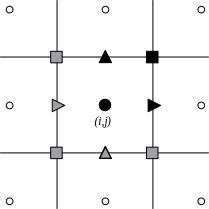
\includegraphics[width=.3\textwidth]{figSStructGridVars}
\caption{%
Grid variables in \hypre{} are referenced by the abstract cell-centered index
to the left and down in 2D (analogously in 3D).  In the figure, index $(i,j)$
is used to reference the variables in black.  The variables in grey---although
contained in the pictured cell---are not referenced by the $(i,j)$ index.}
\label{fig-gridvars}
\end{figure}

The \code{SStruct} interface uses a {\em graph} to allow nearly arbitrary
relationships between part data.  The graph is constructed from stencils or
finite element stiffness matrices plus some additional data-coupling information
set by the \code{GraphAddEntries()} routine.  Two other methods for relating
part data are the \code{GridSetNeighborPart()} and \code{GridSetSharedPart()}
routines, which are particularly well suited for block-structured grid problems.
The latter is useful for finite element codes.

There are five basic steps involved in setting up the linear system to be
solved:
%\begin{enumerate}
\begin{list}{\arabic{enumi}.}{\usecounter{enumi}\setlength{\itemsep}{0in}}
\item set up the grid,
\item set up the stencils (if needed),
\item set up the graph,
\item set up the matrix,
\item set up the right-hand-side vector.
\end{list}
%\end{enumerate}
%In the remainder of this section, we consider three examples: block-structured
%grid problems with stencils (Section~\ref{sec-Block-Structured-Grids});
%block-structured grid problems with finite elements
%(Section~\ref{sec-Block-Structured-Grids-FEM}); and structured adaptive mesh
%refinement problems (Section~\ref{sec-Structured-Adaptive-Mesh-Refinement}).

%-----------------------------------------------------------------------------

\section{Block-Structured Grids with Stencils}
\label{sec-Block-Structured-Grids}

In this section, we describe how to use the \code{SStruct} interface to define
block-structured grid problems.  We do this primarily by example, paying
particular attention to the construction of stencils and the use of the
\code{GridSetNeighborPart()} interface routine.

Consider the solution of the diffusion equation
\begin{equation} \label{eqn-block-diffusion}
- \nabla \cdot (D \nabla u) + \sigma u = f
\end{equation}
on the block-structured grid in Figure~\ref{fig-sstruct-example}, where $D$ is
a scalar diffusion coefficient, and $\sigma \geq 0$.  The discretization
\cite{JEMorel_RMRoberts_MJShashkov_1998} introduces three different types of
variables: cell-centered, $x$-face, and $y$-face.  The three discretization
stencils that couple these variables are also given in the figure.  The
information in this figure is essentially all that is needed to describe the
nonzero structure of the linear system we wish to solve.

\begin{figure}
\centering
\mbox{}\hfill

\includegraphics[width=.45\textwidth]{figSStructExample1a}
\hfill
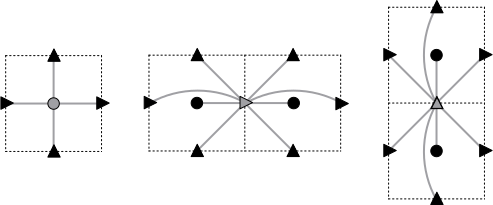
\includegraphics[width=.4\textwidth]{figSStructExample1b}
\hfill\mbox{}
\caption{%
Example of a block-structured grid with five logically-rectangular blocks and
three variables types: cell-centered, $x$-face, and $y$-face.  Discretization
stencils for the cell-centered (left), $x$-face (middle), and $y$-face (right)
variables are also pictured.}
\label{fig-sstruct-example}

\end{figure}
\begin{figure}
\centering
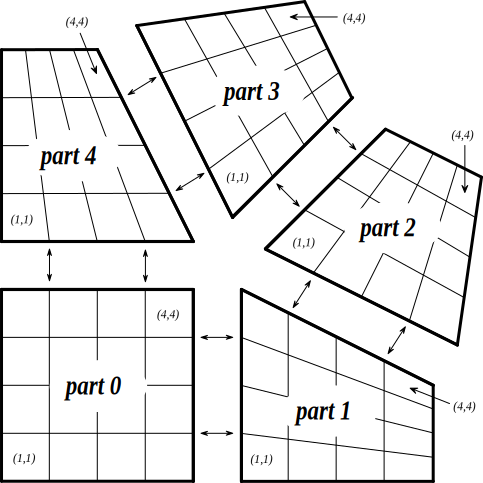
\includegraphics[width=.6\textwidth]{figSStructExample1c}
\caption{%
One possible labeling of the grid in Figure~\ref{fig-sstruct-example}.}
\label{fig-sstruct-example-parts}
\end{figure}

The grid in Figure~\ref{fig-sstruct-example} is defined in terms of five
separate logically-rectangular parts as shown in
Figure~\ref{fig-sstruct-example-parts}, and each part is given a unique label
between 0 and 4.  Each part consists of a single box with lower index $(1,1)$
and upper index $(4,4)$ (see Section~\ref{sec-Struct-Grid}), and the grid data
is distributed on five processes such that data associated with part~$p$ lives
on process~$p$.  Note that in general, parts may be composed out of arbitrary
unions of boxes, and indices may consist of non-positive integers (see
Figure~\ref{fig-struct-boxes}).  Also note that the \code{SStruct} interface
expects a domain-based data distribution by boxes, but the actual distribution
is determined by the user and simply described (in parallel) through the
interface.

\begin{figure}
\centering
\begin{tabular}{@{}c@{}}
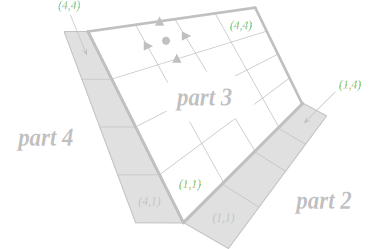
\includegraphics[width=.28\textwidth]{figSStructGrid1} \\ 1
\end{tabular}
\hfill
\begin{tabular}{@{}c@{}}
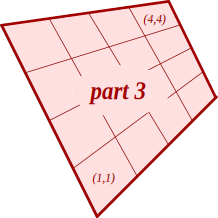
\includegraphics[width=.28\textwidth]{figSStructGrid2} \\ 2
\end{tabular}
\hfill
\begin{tabular}{@{}c@{}}
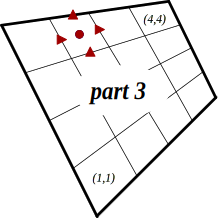
\includegraphics[width=.28\textwidth]{figSStructGrid3} \\ 3
\end{tabular}
\vspace{1em} \\
\begin{tabular}{@{}c@{}}
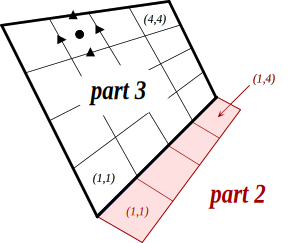
\includegraphics[width=.28\textwidth]{figSStructGrid4} \\ 4
\end{tabular}
\hfill
\begin{tabular}{@{}c@{}}
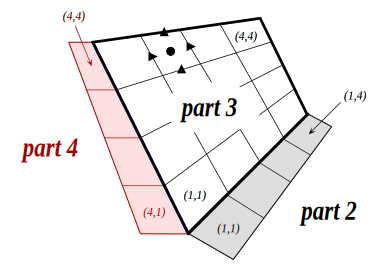
\includegraphics[width=.28\textwidth]{figSStructGrid5} \\ 5
\end{tabular}
\hfill
\begin{tabular}{@{}c@{}}
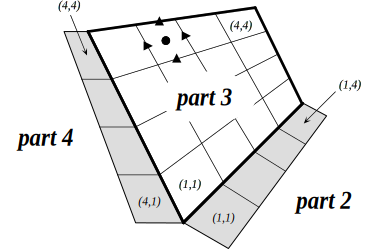
\includegraphics[width=.28\textwidth]{figSStructGrid6} \\ 6
\end{tabular}
\vspace{2em} \\
\begin{minipage}{0.9\textwidth}
\begin{verbatim}
    
    HYPRE_SStructGrid grid;
    int ndim = 2, nparts = 5, nvars = 3, part = 3;
    int extents[][2] = {{1,1}, {4,4}};
    int vartypes[]   = {HYPRE_SSTRUCT_VARIABLE_CELL,
                        HYPRE_SSTRUCT_VARIABLE_XFACE,
                        HYPRE_SSTRUCT_VARIABLE_YFACE};
    int nb2_n_part      = 2,              nb4_n_part      = 4;
    int nb2_exts[][2]   = {{1,0}, {4,0}}, nb4_exts[][2]   = {{0,1}, {0,4}};
    int nb2_n_exts[][2] = {{1,1}, {1,4}}, nb4_n_exts[][2] = {{4,1}, {4,4}};
    int nb2_map[2]      = {1,0},          nb4_map[2]      = {0,1};
    int nb2_dir[2]      = {1,-1},         nb4_dir[2]      = {1,1};

1:  HYPRE_SStructGridCreate(MPI_COMM_WORLD, ndim, nparts, &grid);
    
    /* Set grid extents and grid variables for part 3 */
2:  HYPRE_SStructGridSetExtents(grid, part, extents[0], extents[1]);
3:  HYPRE_SStructGridSetVariables(grid, part, nvars, vartypes);
    
    /* Set spatial relationship between parts 3 and 2, then parts 3 and 4 */
4:  HYPRE_SStructGridSetNeighborPart(grid, part, nb2_exts[0], nb2_exts[1],
       nb2_n_part, nb2_n_exts[0], nb2_n_exts[1], nb2_map, nb2_dir);
5:  HYPRE_SStructGridSetNeighborPart(grid, part, nb4_exts[0], nb4_exts[1],
       nb4_n_part, nb4_n_exts[0], nb4_n_exts[1], nb4_map, nb4_dir);
    
6:  HYPRE_SStructGridAssemble(grid);
    
\end{verbatim}
\end{minipage}
\caption{%
Code on process 3 for setting up the grid in Figure~\ref{fig-sstruct-example}.}
\label{fig-sstruct-grid}
\end{figure}

As with the \code{Struct} interface, each process describes that portion of the
grid that it ``owns'', one box at a time.  Figure~\ref{fig-sstruct-grid} shows
the code for setting up the grid on process~3 (the code for the other processes
is similar).  The ``icons'' at the top of the figure illustrate the result of
the numbered lines of code.  Process~3 needs to describe the data pictured in
the bottom-right of the figure.  That is, it needs to describe part~3 plus some
additional neighbor information that ties part~3 together with the rest of the
grid.  The \code{Create()} routine creates an empty 2D grid object with five
parts that lives on the \code{MPI_COMM_WORLD} communicator.  The
\code{SetExtents()} routine adds a new box to the grid.  The
\code{SetVariables()} routine associates three variables of type cell-centered,
$x$-face, and $y$-face with part~3.

At this stage, the description of the data on part~3 is complete.  However, the
spatial relationship between this data and the data on neighboring parts is not
yet defined.  To do this, we need to relate the index space for part~3 with the
index spaces of parts 2 and~4.  More specifically, we need to tell the interface
that the two grey boxes neighboring part~3 in the bottom-right of
Figure~\ref{fig-sstruct-grid} also correspond to boxes on parts 2 and~4.  This
is done through the two calls to the \code{SetNeighborPart()} routine.  We
discuss only the first call, which describes the grey box on the right of the
figure.  Note that this grey box lives outside of the box extents for the grid
on part~3, but it can still be described using the index-space for part~3
(recall Figure~\ref{fig-struct-boxes}).  That is, the grey box has extents
$(1,0)$ and $(4,0)$ on part~3's index-space, which is outside of part~3's grid.
The arguments for the \code{SetNeighborPart()} call are simply the lower and
upper indices on part~3 and the corresponding indices on part~2.  The final two
arguments to the routine indicate that the positive $x$-direction on part~3
(i.e., the $i$ component of the tuple $(i,j)$) corresponds to the positive
$y$-direction on part~2 and that the positive $y$-direction on part~3
corresponds to the positive $x$-direction on part~2.

The \code{Assemble()} routine is a collective call (i.e., must be called on all
processes from a common synchronization point), and finalizes the grid
assembly, making the grid ``ready to use''.

With the neighbor information, it is now possible to determine where off-part
stencil entries couple.  Take, for example, any shared part boundary such as
the boundary between parts 2 and~3.  Along these boundaries, some stencil
entries reach outside of the part.  If no neighbor information is given, these
entries are effectively zeroed out, i.e., they don't participate in the
discretization.  However, with the additional neighbor information, when a
stencil entry reaches into a neighbor box it is then coupled to the part
described by that neighbor box information.

Another important consequence of the use of the \code{SetNeighborPart()} routine
is that it can declare variables on different parts as being the same.  For
example, the face variables on the boundary of parts 2 and~3 are recognized as
being shared by both parts (prior to the \code{SetNeighborPart()} call, there
were two distinct sets of variables).  Note also that these variables are of
different types on the two parts; on part~2 they are $x$-face variables, but on
part~3 they are $y$-face variables.

For brevity, we consider only the description of the $y$-face stencil in
Figure~\ref{fig-sstruct-example}, i.e. the third stencil in the figure.  To do
this, the stencil entries are assigned unique labels between 0 and 8 and their
``offsets'' are described relative to the ``center'' of the stencil.  This
process is illustrated in Figure \ref{fig-sstruct-stencil}.  Nine calls are
made to the routine \code{HYPRE_SStructStencilSetEntry()}.  As an example, the
call that describes stencil entry 5 in the figure is given the entry number~5,
the offset $(-1,0)$, and the identifier for the $x$-face variable (the variable
to which this entry couples).  Recall from Figure~\ref{fig-gridvars} the
convention used for referencing variables of different types.  The geometry
description uses the same convention, but with indices numbered relative to the
referencing index $(0,0)$ for the stencil's center.
Figure~\ref{fig-sstruct-graph} shows the code for setting up the graph .

\begin{figure}
\centering
\mbox{}\hfill
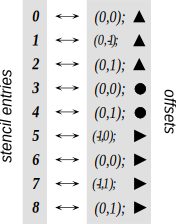
\includegraphics[width=.25\textwidth]{figSStructStenc0}
\hfill
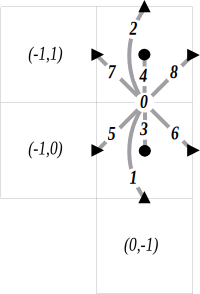
\includegraphics[width=.2\textwidth]{figSStructStenc1}
\hfill\mbox{}
\caption{%
Assignment of labels and geometries to the $y$-face stencil in
Figure~\ref{fig-sstruct-example}.}
\label{fig-sstruct-stencil}
\end{figure}

\begin{figure}
\centering
\begin{tabular}{@{}c@{}}
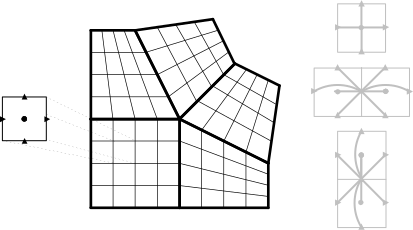
\includegraphics[width=.32\textwidth]{figSStructGraph1}\vspace{-.5em} \\ 1
\end{tabular}
\hfill
\begin{tabular}{@{}c@{}}
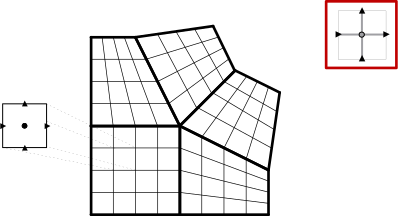
\includegraphics[width=.32\textwidth]{figSStructGraph2}\vspace{-.5em} \\ 2
\end{tabular}
\hfill
\begin{tabular}{@{}c@{}}
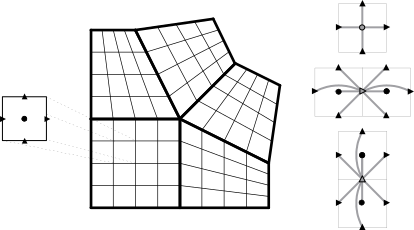
\includegraphics[width=.32\textwidth]{figSStructGraph5}\vspace{-.5em} \\ 3
\end{tabular}
\vspace{1em} \\
\begin{minipage}{0.9\textwidth}
\begin{verbatim}
    
    HYPRE_SStructGraph graph;
    HYPRE_SStructStencil c_stencil, x_stencil, y_stencil;
    int c_var = 0, x_var = 1, y_var = 2;
    int part;
    
1:  HYPRE_SStructGraphCreate(MPI_COMM_WORLD, grid, &graph);
    
    /* Set the cell-centered, x-face, and y-face stencils for each part */
    for (part = 0; part < 5; part++)
    {
2:     HYPRE_SStructGraphSetStencil(graph, part, c_var, c_stencil);
       HYPRE_SStructGraphSetStencil(graph, part, x_var, x_stencil);
       HYPRE_SStructGraphSetStencil(graph, part, y_var, y_stencil);
    }
    
3:  HYPRE_SStructGraphAssemble(graph);

\end{verbatim}
\end{minipage}
\caption{%
Code on process 3 for setting up the graph for Figure~\ref{fig-sstruct-example}.}
\label{fig-sstruct-graph}
\end{figure}

With the above, we now have a complete description of the nonzero structure for
the matrix.  The matrix coefficients are then easily set in a manner similar to
what is described in Section~\ref{sec-Struct-Matrix} using routines
\code{MatrixSetValues()} and \code{MatrixSetBoxValues()} in the \code{SStruct}
interface.  As before, there are also \code{AddTo} variants of these routines.
Likewise, setting up the right-hand-side is similar to what is described in
Section~\ref{sec-Struct-RHS}.  See the \hypre{} reference manual for details.

An alternative approach for describing the above problem through the interface
is to use the \code{GraphAddEntries()} routine instead of the
\code{GridSetNeighborPart()} routine.  In this approach, the five parts would be
explicitly ``sewn'' together by adding non-stencil couplings to the matrix
graph.  The main downside to this approach for block-structured grid problems
is that variables along block boundaries are no longer considered to be the
same variables on the corresponding parts that share these boundaries.  For
example, any face variable along the boundary between parts 2 and~3 in
Figure~\ref{fig-sstruct-example} would represent two different variables that
live on different parts.  To ``sew'' the parts together correctly, we would
need to explicitly select one of these variables as the representative that
participates in the discretization, and make the other variable a dummy
variable that is decoupled from the discretization by zeroing out appropriate
entries in the matrix.  All of these complications are avoided by using the
\code{GridSetNeighborPart()} for this example.

%-----------------------------------------------------------------------------

\section{Block-Structured Grids with Finite Elements}
\label{sec-Block-Structured-Grids-FEM}

In this section, we describe how to use the \code{SStruct} interface to define
block-structured grid problems with finite elements.  We again do this by
example, paying particular attention to the use of the \code{FEM} interface
routines and the \code{GridSetSharedPart()} routine.  See example code
\file{ex14.c} for a complete implementation.

Consider a nodal finite element (FEM) discretization of the Laplace equation on
the star-shaped grid in Figure~\ref{fig-sstruct-fem-example}.  The local FEM
stiffness matrix in the figure describes the coupling between the grid
variables.  Although we could still describe this problem using stencils as in
Section~\ref{sec-Block-Structured-Grids}, an FEM-based approach (available in
\hypre{} version \code{2.6.0b} and later) is a more natural alternative.

\begin{figure} [t]
\centering

\includegraphics[width=.54\textwidth]{figSStructExample3a}
\hfill
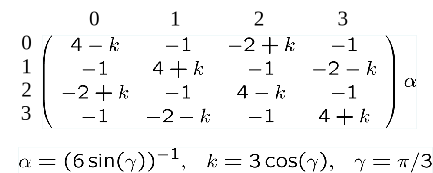
\includegraphics[width=.44\textwidth]{figSStructExample3b}
\caption{%
Example of a star-shaped grid with six logically-rectangular blocks and one
nodal variable.  Each block has an angle at the origin given by $\gamma=\pi/3$.
The finite element stiffness matrix (right) is given in terms of the pictured
variable ordering (left).}
\label{fig-sstruct-fem-example}
\end{figure}

%\begin{figure}
%\centering
%
\includegraphics[width=.5\textwidth]{figSStructExample3c}
%\caption{%
%One possible labeling of the grid in Figure~\ref{fig-sstruct-fem-example}.}
%\label{fig-sstruct-fem-example-parts}
%\end{figure}

The grid in Figure~\ref{fig-sstruct-fem-example} is defined in terms of six
separate logically-rectangular parts, and each part is given a unique label
between 0 and 5.  Each part consists of a single box with lower index $(1,1)$
and upper index $(9,9)$, and the grid data is distributed on six processes such
that data associated with part~$p$ lives on process~$p$.

\begin{figure}
\centering
\begin{tabular}{@{}c@{}}
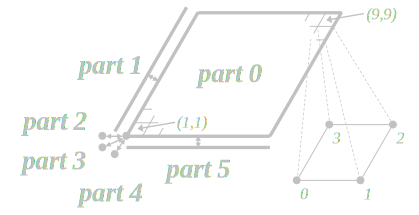
\includegraphics[width=.32\textwidth]{figSStructGridFEM1} \\ 1
\end{tabular}
\hfill
\begin{tabular}{@{}c@{}}

\includegraphics[width=.32\textwidth]{figSStructGridFEM2} \\ 2
\end{tabular}
\hfill
\begin{tabular}{@{}c@{}}
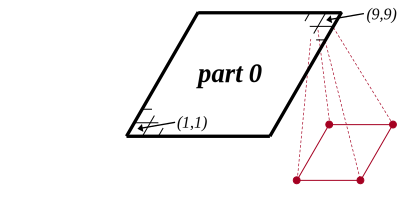
\includegraphics[width=.32\textwidth]{figSStructGridFEM3} \\ 3
\end{tabular}
\vspace{1em} \\
\begin{tabular}{@{}c@{}}
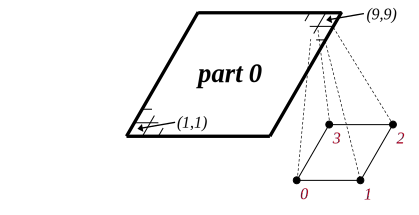
\includegraphics[width=.32\textwidth]{figSStructGridFEM4} \\ 4
\end{tabular}
\hfill
\begin{tabular}{@{}c@{}}
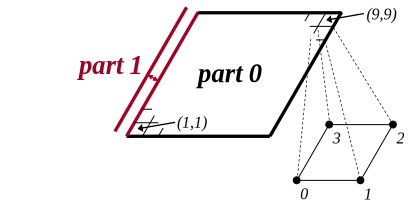
\includegraphics[width=.32\textwidth]{figSStructGridFEM5} \\ 5
\end{tabular}
\hfill
\begin{tabular}{@{}c@{}}

\includegraphics[width=.32\textwidth]{figSStructGridFEM6} \\ 6
\end{tabular}
\vspace{2em} \\
\begin{minipage}{0.9\textwidth}
\begin{verbatim}
    
    HYPRE_SStructGrid grid;
    int ndim = 2, nparts = 6, nvars = 1, part = 0;
    int ilower[2]    = {1,1}, iupper[2] = {9,9};
    int vartypes[]   = {HYPRE_SSTRUCT_VARIABLE_NODE};
    int ordering[12] = {0,-1,-1,  0,+1,-1,  0,+1,+1,  0,-1,+1};

    int s_part   = 2;
    int ilo[2]   = {1,1}, iup[2]   = {1,9}, offset[2]   = {-1,0};
    int s_ilo[2] = {1,1}, s_iup[2] = {9,1}, s_offset[2] = {0,-1};
    int map[2]   = {1,0};
    int dir[2]   = {-1,1};

1:  HYPRE_SStructGridCreate(MPI_COMM_WORLD, ndim, nparts, &grid);
    
    /* Set grid extents, grid variables, and FEM ordering for part 0 */
2:  HYPRE_SStructGridSetExtents(grid, part, ilower, iupper);
3:  HYPRE_SStructGridSetVariables(grid, part, nvars, vartypes);
4:  HYPRE_SStructGridSetFEMOrdering(grid, part, ordering);

    /* Set shared variables for parts 0 and 1 (0 and 2/3/4/5 not shown) */
5:  HYPRE_SStructGridSetSharedPart(grid, part, ilo, iup, offset,
       s_part, s_ilo, s_iup, s_offset, map, dir);

6:  HYPRE_SStructGridAssemble(grid);
    
\end{verbatim}
\end{minipage}
\caption{%
Code on process 0 for setting up the grid in Figure~\ref{fig-sstruct-fem-example}.}
\label{fig-sstruct-fem-grid}
\end{figure}

As in Section~\ref{sec-Block-Structured-Grids}, each process describes that
portion of the grid that it ``owns'', one box at a time.
Figure~\ref{fig-sstruct-fem-grid} shows the code for setting up the grid on
process~0 (the code for the other processes is similar).  The ``icons'' at the
top of the figure illustrate the result of the numbered lines of code.
Process~0 needs to describe the data pictured in the bottom-right of the figure.
That is, it needs to describe part~0 plus some additional information about
shared data with other parts on the grid.  The \code{SetFEMOrdering()} routine
sets the ordering of the unknowns in an element (an element is always a grid
cell in \hypre{}).  This determines the ordering of the data passed into the
routines \code{MatrixAddFEMValues()} and \code{VectorAddFEMValues()} discussed
later.

At this point, the layout of the data on part~0 is complete, but there is no
relationship to the rest of the grid.  To couple the parts, we need to tell
\hypre{} that some of the boundary variables on part~0 are shared with other
parts, i.e., they are the same as some of the variables on other parts.  This is
done through five calls to the \code{SetSharedPart()} routine.  Only the first
call is shown in the figure; the other four calls are similar.  The arguments to
this routine are the same as \code{SetNeighborPart()} with the addition of two
new offset arguments, named \code{offset} and \code{s_offset} in the figure.
Each offset represents a pointer from the cell center to one of the following:
all variables in the cell (no nonzeros in offset); all variables on a face (only
1 nonzero); all variables on an edge (2 nonzeros); all variables at a point (3
nonzeros).  The two offsets must be consistent with each other.

The graph is set up similarly to Figure~\ref{fig-sstruct-graph}, except that the
stencil calls are replaced by calls to \code{GraphSetFEM()}.  The nonzero
pattern of the stiffness matrix can also be set by calling the optional routine
\code{GraphSetFEMSparsity()}.

Matrix and vector values are set one element at a time.  For the example in this
section, calls on part~0 would have the following form:
\begin{verbatim}
   int part = 0;
   int index[2] = {i,j};
   double m_values[16] = {...};
   double v_values[4]  = {...};
   
   HYPRE_SStructMatrixAddFEMValues(A, part, index, m_values);
   HYPRE_SStructVectorAddFEMValues(v, part, index, v_values);
\end{verbatim}
Here, \code{m_values} contains local stiffness matrix values and \code{v_values}
contains local variable values.  The global matrix and vector are assembled
internally by \hypre{}, using the shared variables to couple the parts.

%-----------------------------------------------------------------------------

\section{Structured Adaptive Mesh Refinement}
\label{sec-Structured-Adaptive-Mesh-Refinement}

We now briefly discuss how to use the \code{SStruct} interface in a structured
AMR application.  Consider Poisson's equation on the simple cell-centered
example grid illustrated in Figure \ref{fig-sstruct-samr-grid}.  For structured
AMR applications, each refinement level should be defined as a unique part.
There are two parts in this example: part~0 is the global coarse grid and
part~1 is the single refinement patch.  Note that the coarse unknowns
underneath the refinement patch (gray dots in Figure
\ref{fig-sstruct-samr-grid}) are not real physical unknowns; the solution in
this region is given by the values on the refinement patch.  In setting up the
composite grid matrix \cite{SFMcCormick_1989a} for \hypre{} the equations for
these ``dummy'' unknowns should be uncoupled from the other unknowns (this can
easily be done by setting all off-diagonal couplings to zero in this region).

\begin{figure}
\centering
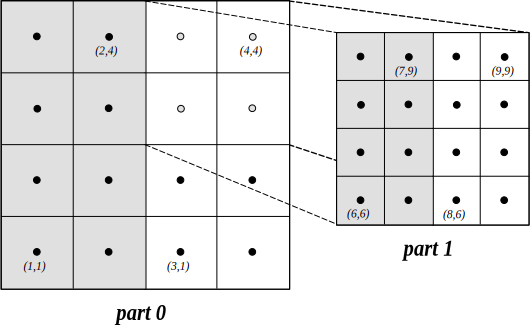
\includegraphics[width=.7\textwidth]{figSStructExample2a}
\caption{%
Structured AMR grid example. Shaded regions correspond to process~0, unshaded
to process~1.  The grey dots are dummy variables.}
\label{fig-sstruct-samr-grid}
\end{figure}

In the example, parts are distributed across the same two processes with
process 0 having the ``left'' half of both parts.  The composite grid is then
set up part-by-part by making calls to \code{GridSetExtents()} just as was done
in Section~\ref{sec-Block-Structured-Grids} and Figure~\ref{fig-sstruct-grid}
(no \code{SetNeighborPart} calls are made in this example).  Note that in the
interface there is no required rule relating the indexing on the refinement
patch to that on the global coarse grid; they are separate parts and thus each
has its own index space.  In this example, we have chosen the indexing such
that refinement cell $(2i,2j)$ lies in the lower left quadrant of coarse cell
$(i,j)$.  Then the stencil is set up.  In this example we are using a finite
volume approach resulting in the standard 5-point stencil in
Figure~\ref{fig-struct-stencil-b} in both parts.

The grid and stencil are used to define all intra-part coupling in the graph,
the non-zero pattern of the composite grid matrix.  The inter-part coupling at
the coarse-fine interface is described by \code{GraphAddEntries()} calls.  This
coupling in the composite grid matrix is typically the composition of an
interpolation rule and a discretization formula.  In this example, we use a
simple piecewise constant interpolation, i.e. the solution value in a coarse
cell is equal to the solution value at the cell center.  Then the flux across a
portion of the coarse-fine interface is approximated by a difference of the
solution values on each side.  As an example, consider approximating the flux
across the left interface of cell $(6,6)$ in Figure
\ref{fig-sstruct-samr-stencil}.  Let $h$ be the coarse grid mesh size, and
consider a local coordinate system with the origin at the center of cell
$(6,6)$.  We approximate the flux as follows
\begin{eqnarray}
\int_{-h/4}^{h/4}{u_x(-h/4,s)} ds
& \approx & \frac{h}{2} u_x(-h/4,0)
  \approx \frac{h}{2} \frac{u(0,0)-u(-3h/4,0)}{3h/4} \\
& \approx & \frac{2}{3} (u_{6,6}-u_{2,3}) \nonumber .
\end{eqnarray} 
The first approximation uses the midpoint rule for the edge integral, the second
uses a finite difference formula for the derivative, and the third the piecewise
constant interpolation to the solution in the coarse cell.  This means that the
equation for the variable at cell $(6,6)$ involves not only the stencil
couplings to $(6,7)$ and $(7,6)$ on part~1 but also non-stencil couplings to
$(2,3)$ and $(3,2)$ on part~0.  These non-stencil couplings are described by
\code{GraphAddEntries()} calls.  The syntax for this call is simply the part and
index for both the variable whose equation is being defined and the variable to
which it couples.  After these calls, the non-zero pattern of the matrix (and
the graph) is complete.  Note that the ``west'' and ``south'' stencil couplings
simply ``drop off'' the part, and are effectively zeroed out (currently, this is
only supported for the \code{HYPRE_PARCSR} object type, and these values must be
manually zeroed out for other object types; see \code{MatrixSetObjectType()} in
the reference manual).

\begin{figure}
\centering
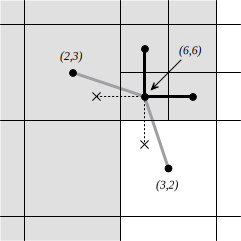
\includegraphics[width=.4\textwidth]{figSStructExample2b}
\caption{%
Coupling for equation at corner of refinement patch. Black lines
(solid and broken) are stencil couplings. Gray line are non-stencil
couplings.}
\label{fig-sstruct-samr-stencil}
\end{figure}

The remaining step is to define the actual numerical values for the composite
grid matrix.  This can be done by either \code{MatrixSetValues()} calls to set
entries in a single equation, or by \code{MatrixSetBoxValues()} calls to set
entries for a box of equations in a single call.  The syntax for the
\code{MatrixSetValues()} call is a part and index for the variable whose
equation is being set and an array of entry numbers identifying which entries
in that equation are being set.  The entry numbers may correspond to stencil
entries or non-stencil entries.

%\chapter{Finite Element Interface}
\label{ch-FEI}

\section{Introduction}

User applications access the \hypre{} linear solvers via a pipeline of
two interfaces - user to finite element interface (called {\sf FEI}),
and the finite element to linear solver interface (called 
{\sf LinearSystemCore}). The purpose of {\sf FEI} is to allow users 
to submit the global matrices in the form of element connectivities, 
element stiffness matrices, element loads, and boundary conditions. 
These element information are processed by an implementation of the 
{\sf FEI} (see \cite{FEI-ref}) which loads the global matrix and right
hand side vectors to the linear solver libraries via the 
{\sf LinearSystemCore} interface.
The {\sf LinearSystemCore} interface also facilitates interfacing 
multiple linear system solver packages (such as PetSC or Aztec)
with little change in the user code.

The specification of the {\sf FEI} and its implementation was first
developed at Sandia. A simplified implementation has been implemented
at LLNL in \hypre{}'s finite element module. In the next section, we 
describe the basic {\sf FEI} functions and a sample program to 
demonstrate how to use them. 
%A brief description of \hypre{}'s 
%internal data structure and solver capabilities is presented in 
%Section 5.3.  Associated with \hypre{}'s finite element interface is 
%an FE-based gray-box multilevel preconditioning module called 
%{\sf MLI} which provides fast multilevel preconditioners.
%A description of the {\sf MLI} is given in Section 5.4.
%In Section 5.5, we describe the available options for using \hypre{}'s
%rich solver capabilities. 
Users who prefer to create their own finite
element packages but would like to use the \hypre{} solvers can link their
packages to \hypre{} via the {\sf LinearSystemCore}. A description
of this interface is given in Section 4.3.  Finally, some installation 
and usage issues are discussed in Section 4.4.

\section{A Brief Description of The Finite Element Interface}

Embedded in application finite element codes are data structures
storing element connectivities, element stiffness matrices, element
loads, boundary conditions, nodal coordinates, etc. An implicit finite
element problem can be solved by assembling the global stiffness matrix
and the corresponding right hand side vector, and then calling linear
solver to calculate the solution. The first step in this process is 
thus to instantiate an {\sf FEI} object by
\begin{tabbing}
\hspace{0.5in} \= {\sf feiPtr = new FEI\_Implementation(mpiComm);}
\end{tabbing}
where {\sf mpiComm} is an MPI communicator (e.g. {\sf MPI\_COMM\_WORLD}).
Next, various finite element information need to be sent into the {\sf FEI}
object.

The first entity to be submitted to the {\sf FEI} is {\it field} information. 
A {\it field} has an identifier called {\it fieldID} and a rank or
{\it fieldSize} (number of degree of freedom). For example, for a simple
3D incompressible Navier Stokes equation, the nodal variable is the velocity
vector which has $3$ degrees of freedom; and the element variable (constant
over the element) is the pressure (scalar). If these are the only variables,
and if we assign {\it fieldID} $7$ and $8$ to them, respectively, then the
finite element field information can be set up by
\begin{tabbing}
\hspace{0.5in} \= {\sf nFields = 2;} \\
               \> {\sf fieldID = new int[nFields];} \\
               \> {\sf fieldID[0] = $7$; /* velocity vector */} \\
               \> {\sf fieldID[1] = $8$; /* pressure */} \\
               \> {\sf fieldSize = new int[nFields];} \\
               \> {\sf fieldSize[0] = $3$; /* velocity vector */} \\
               \> {\sf fieldSize[1] = $1$; /* pressure */ } \\
               \> {\sf feiPtr$->$initFields(nFields, fieldSize, fieldID);}
\end{tabbing}

Once the field information has been established, we are ready to initialize
an element block. An element block is characterized by the block identifier,
the number of elements, the number of nodes per element, the nodal fields 
and the element fields (fields that have been defined previously). Suppose 
we use $1000$ hexahedral elements in the element block $0$, the setup 
consists of
\begin{tabbing}
\hspace{0.5in} \= {\sf elemBlkID = 0;} \\
               \> {\sf nElems = 1000;} \\
               \> {\sf elemNNodes = 8; /* number of nodes per element */} \\
               \> {\sf nodeNFields = 1; /* nodal field - velocity */} \\
               \> {\sf nodeFieldIDs = new[nodeNFields];} \\
               \> {\sf nodeFieldIDs[0] = fieldID[0]; /* velocity */ } \\
               \> {\sf elemNFields = 1; /* element field - pressure */} \\
               \> {\sf elemFieldIDs = new[elemNFields];} \\
               \> {\sf elemFieldIDs[0] = fieldID[1]; /* pressure */ } \\
 \> {\sf feiPtr$->$initElemBlock(elemBlkID, nElems, elemNNodes, nodeNFields, nodeFieldIDs,}\\
 \> \hspace{1.0in} {\sf elemNFields, elemFieldIDs, 0);} 
\end{tabbing}
The last argument is to specify how the dependent variables are arranged in
the element matrices. A value of $0$ indicates that each variable is to be
arranged in a separate block (as opposed to interleaving).

In a parallel environment, each processor has one or more element blocks.
Unless the element blocks are all disjoint, some of the element blocks
share a common set of nodes on the subdomain boundaries. To facilitate
setting up interprocessor communications, shared nodes between subdomains
on different processors are to be identified and sent to the {\sf FEI}.
Hence, each node in the whole domain is assigned a unique global
identifier. The shared node list on each processor contains a subset
of the global node list
corresponding to the local nodes that are shared with the other processors.
The syntax for setting up the shared nodes is
\begin{tabbing}
\hspace{0.5in} \= {\sf feiPtr$->$initSharedNodes(nShared, sharedIDs, sharedLengs, sharedProcs);}
\end{tabbing}
This completes the initialization phase, and a completion signal is sent to
the {\sf FEI} via
\begin{tabbing}
\hspace{0.5in} \= {\sf feiPtr$->$initComplete();}
\end{tabbing}

Next we begin the {\it load} phase. The first entity for loading is the
nodal boundary conditions. Here we need to specify the number of boundary
equations and the boundary values given by {\sf alpha, beta}, and {\sf gamma}.  Depending whether the boundary conditions are Dirichlet, Neumann, or mixed,
the three values should be passed into the {\sf FEI} accordingly. 

The element stiffness matrices are to be loaded in the next step. We need
to specify the element number $i$, the element block to which element $i$
belongs, the element connectivity information, the element load, and the
element matrix format. The element connectivity specifies a set of $8$ node
global IDs (for hexahedral elements), and the element load is the load or
force for each degree of freedom.  The element format specifies how the
equations are arranged (similar to the interleaving scheme mentioned above).
The calling sequence for loading element stiffness matrices is
\begin{tabbing}
\hspace{0.5in} \= {\sf for (iE = 0; iE < nElems; iE++)} \\
 \> \hspace{0.5in} {\sf feiPtr$->$sumInElem(elemBlkID, elemID, elemConn[iE], elemStiff[iE],} \\
 \> \hspace{1.5in} {\sf elemLoads[iE], elemFormat);}
\end{tabbing}
Again, to complete the loading phase, a completion signal is sent to 
the {\sf FEI} via
\begin{tabbing}
\hspace{0.5in} \= {\sf feiPtr$->$loadComplete();}
\end{tabbing}
 
Now the global stiffness matrix and the corresponding right hand side
have been assembled. Before the linear system is solved, a number of 
solver parameters have to be passed into the {\sf FEI}. A detailed description
of the solver parameters is given in Section 3. An example is given below
\begin{tabbing}
\hspace{0.5in} \= {\sf nParams = 5;} \\
               \> {\sf paramStrings = new char*[nParams];} \\
               \> {\sf for (i = 0; i < nParams; i++) }\\
               \> \hspace{0.5in} {\sf paramStrings[i] = new char[100];} \\
               \> {\sf strcpy(paramStrings[0], "solver cg");} \\
               \> {\sf strcpy(paramStrings[1], "preconditioner diag");} \\
               \> {\sf strcpy(paramStrings[2], "maxiterations 100");} \\
               \> {\sf strcpy(paramStrings[3], "tolerance 1.0e-6");} \\
               \> {\sf strcpy(paramStrings[4], "outputLevel 1");} \\
               \> {\sf feiPtr$->$parameters(nParams, paramStrings);} 
\end{tabbing}

To solve the linear system of equations, we call
\begin{tabbing}
\hspace{0.5in} \= {\sf feiPtr$->$solve(\&status);}
\end{tabbing}
where {\sf status} is returned from the {\sf FEI} indicating whether
the solve is successful. Finally, the solution can be retrieved by
\begin{tabbing}
\hspace{0.5in} \= {\sf feiPtr$->$getBlockNodeSolution(elemBlkID, nNodes, nodeIDList, solnOffsets, solnValues);}
\end{tabbing}
where {\sf solnOffsets[i]} is the index pointing to the first location 
where the variables at node $i$ is returned in {\sf solnValues}.

\section{The LinearSystemCore Interface}

As described before, users who prefer to create their own finite element
interface package can also take advantage of the rich solver capabilities
in \hypre{}. In this section we show how to access {\sf HYPRE\_LinSysCore}'s
internal solver directly.  Users who choose this path need first to 
construct an array (say, {\sf eqnOffsets} describing the matrix row
partitioning across all processors (so {\sf eqnOffsets[p]} and
{\sf eqnOffset[p+1]} have the starting and ending row indices for processor
p). Furthermore, suppose the local submatrix has been constructed as a
compressed sparse row (CSR) matrix in the {\sf ia, ja, val} arrays. 
The following program segment describes the function calls to set up
the internal matrix and solve the linear system.

\begin{tabbing}
\hspace{0.5in} \= {\sf Program Segment} \\[1mm]
\> {\sf startRow = eqnOffsets[mypid];} \\
\> {\sf endRow = eqnOffsets[mypid+1] - 1;} \\
\> {\sf nrows = endRow - startRow + 1} \\
\> {\sf for ( i = startRow; i $<=$ endRow; i++ ) $\{$ } \\
\> \hspace{0.3in} \= {\sf ncnt = ia[i+1] - ia[i];} \\
\> \> {\sf rowLengths[i-startRow] = ncnt;} \\
\> \> {\sf colIndices[i-startRow] = new int[ncnt];} \\
\> \> {\sf k = 0;} \\
\> \> {\sf for (j = ia[i]; j < ia[i+1]; j++) colIndices[i-startRow][k++] = ja[j];}\\
\> \} \\
\> {\sf HYPRE\_LinSysCore\_create(\&lsc, MPI\_COMM\_WORLD);} \\
\> {\sf HYPRE\_setGlobalOffsets(lsc, nrows, NULL, eqnOffsets, NULL);} \\
\> {\sf HYPRE\_setMatrixStructure(lsc, colIndices, rowLengths, NULL, NULL, NULL);} \\
\> {\sf for ( i = startRow; i <= endRow; i++ ) $\{$ } \\
\> \> {\sf ncnt = ia[i+1] - ia[i];} \\
\> \> {\sf HYPRE\_sumIntoSystemMatrix(lsc, i, ncnt, \&val[ia[i]], \&ja[ia[i]]);}\\
\> \> {\sf HYPRE\_sumIntoRHSVector(1, \&rhs[i], \&i);} \\
\> \} \\
\> {\sf HYPRE\_matrixLoadComplete();}\\
\> {\sf strcpy(paramString, "solver gmres");} \\
\> {\sf HYPRE\_parameters(1, \&paramString);} \\
\> {\sf strcpy(paramString, "preconditioner boomeramg");} \\
\> {\sf HYPRE\_parameters(1, \&paramString);} \\
\> {\sf HYPRE\_launchSolver(\&status, \&iterations);}
\end{tabbing}

A list of available functions is given in the following.

\begin{tabbing}
{\sf HYPRE\_LinSysCore\_create(LinSysCore **lsc, MPI\_Comm comm)} \\[1mm]
{\sf HYPRE\_LinSysCore\_destroy(LinSysCore **lsc)} \\[1mm]
{\sf HYPRE\_parameters(LinSysCore *lsc, int nParams, char **params)} \\[1mm]
{\sf HYPRE\_setGlobalOffsets(LinSysCore* lsc, int leng, int* nodeOffsets,} \\
\hspace{1.0in} {\sf int* eqnOffsets, int* blkEqnOffsets)} \\[1mm]
{\sf HYPRE\_setMatrixStructure(LinSysCore *lsc, int** ptColIndices,} \\
\hspace{1.0in} {\sf int* ptRowLengths, int** blkColIndices, int* blkRowLengths, int* ptRowsPerBlkRow)} \\[1mm]
{\sf HYPRE\_resetMatrixAndVector(LinSysCore *lsc, double val)} \\[1mm]
{\sf HYPRE\_resetMatrix(LinSysCore *lsc, double val)} \\[1mm]
{\sf HYPRE\_resetRHSVector(LinSysCore *lsc, double val)} \\[1mm]
{\sf HYPRE\_sumIntoSystemMatrix(LinSysCore *lsc, int numPtRows, const int* ptRows,}\\
\hspace{1.0in} {\sf int numPtCols, const int* ptCols, int numBlkRows, const int* blkRows,} \\
\hspace{1.0in} {\sf int numBlkCols, const int* blkCols, const double* const* values)} \\[1mm]
{\sf HYPRE\_sumIntoRHSVector(LinSysCore *lsc, int num, const double* values, const int* indices)} \\[1mm]
{\sf HYPRE\_matrixLoadComplete(LinSysCore *lsc)} \\[1mm]
{\sf HYPRE\_enforceEssentialBC(LinSysCore *lsc, int* globalEqn, double* alpha,
                             double* gamma, int leng)} \\[1mm]

{\sf HYPRE\_enforceRemoteEssBCs(LinSysCore *lsc,int numEqns,int* globalEqns, int** colIndices,} \\
\hspace{1.0in} {\sf int* colIndLen, double** coefs)} \\[1mm]

{\sf HYPRE\_enforceOtherBC(LinSysCore *lsc, int* globalEqn, double* alpha, double *beta} \\
\hspace{1.0in} {\sf double* gamma, int leng)} \\[1mm]

{\sf HYPRE\_putInitialGuess(LinSysCore *lsc, const int* eqnNumbers,
                          const double* values, int leng)} \\[1mm]
{\sf HYPRE\_getSolution(LinSysCore *lsc, double *answers, int leng)} \\[1mm]

{\sf HYPRE\_getSolnEntry(LinSysCore *lsc, int eqnNumber, double *answer)} \\[1mm]

{\sf HYPRE\_formResidual(LinSysCore *lsc, double *values, int leng)} \\[1mm]

{\sf HYPRE\_launchSolver(LinSysCore *lsc, int *solveStatus, int *iter)} \\[1mm]
\end{tabbing}

\section{HYPRE LinearSystemCore Installation}

The ultimate objective is for application users to have immediate access
to the latest FEI/\hypre{} library files on different computing platforms
via public {\sf lib} directories.  While this feature is forthcoming, careful 
version control is needed for users to keep track of capabilities and bug fixes 
for different installations.  Users who would like to set up the FEI/\hypre{}
on their own should do the following :

\begin{enumerate}

\item obtain the \hypre{} and the Sandia FEI source codes (alternatively, use
      the {\sf FEI} implementation in \hypre{}),
\item compile Sandia's {\sf FEI} (fei-2.5.0) to create the
      {\sf libfei\_base.a} file.
\item compile \hypre{} 
\begin{enumerate}
\item download \hypre{} from the web, ungzip and untar it
\item go into the {\sf linear\_solvers} directory
\item do a 'configure' with the {\sf --with-fei-inc-dir} option set to
      the {\sf FEI} include directory plus other compile options
\item compile with {\sf make install} to create the
      {\sf libHYPRE\_LSI*} file in the {\sf linear\_solvers/hypre/lib}
      directory.
\end{enumerate}
\item call the {\sf FEI} functions in your application code (example given
      previously)
\begin{enumerate}
\item include {\sf cfei\-hypre.h} in your file 
\item include {\sf FEI\_Implementation.h} in your file 
\item make sure your application has an {\sf include} and an {\sf lib} path 
      to the {\sf include} and {\sf lib} directories created above. 
\end{enumerate}

\end{enumerate}

%\subsection{Linking with the library files}

To link the {\sf FEI} and \hypre{} into the executable, the following has to be
attached to the linking command :

\begin{tabbing}
\hspace{0.5in} \= {\sf -L\$$\{$LIBPATHS$\}$ -lfei\_base -lHYPRE\_LSI} 
\end{tabbing}
along with all the other libraries (Note : the order in which the libraries are
listed may be important), where {\sf LIBPATHS} are where 
the \hypre{} and {\sf FEI} libraray files can be found.  

Since some of these library files make calls to LAPACK and BLAS functions, 
the corresponding libraries need to be linked along with (placed after) these 
library files.  
%For example, on the DEC cluster, it suffices to link
%with the {\sf dxml} library, (So {\sf -ldxml} is placed after the above link
%sequence, with {\sf -lm} placed after {\sf -ldxml}.) while the {\it essl}
%library can be used on the blue machine. If {\sf SuperLU} is also needed,
%{\sf -lHYPRE\_superlu} should be placed immediately after {\sf HYPRE\_LSI}.

%\subsection{Some more caveats for application developers}

Building an application executable often requires linking with many different
software packages, and many software packages use some LAPACK and/or BLAS
functions.  In order to alleviate the problem of multiply defined functions
at link time, it is recommended that all software libraries are stripped of
all LAPACK and BLAS function definitions.  These LAPACK and BLAS functions 
should then be resolved at link time by linking with the system LAPACK and
BLAS libraries (e.g. dxml on DEC cluster).  Both \hypre{} and SuperLU were
built with this in mind.  However, some other software library files needed
may have the BLAS functions defined in them.  To avoid the problem of
multiply defined functions, it is recommended that the offending library
files be stripped of the BLAS functions.

%\subsection{Comments about the FEI/\hypre{} Interface and Contacts}

%Comments about \hypre{}'s finite element interface can be directed
%to Charles Tong (925-422-3411, chtong@llnl.gov).


%%==========================================================================
\chapter{The IJ Linear System Interface}
\label{IJ}

The {\bf IJ linear system (IJ)} interface is the lowest common
denominator
for enumeration of an {\bf unaugmented} linear system of equations
to be solved by {\slshape hypre} and cooperative packages.
No underlying assumptions are made about the sparsity pattern of
a linear system passed through the IJ interface.
Like all Hypre interfaces, it is designed
to insulate the user from underlying implementation details.

Just to define an {\bf augmented} linear system, an example would be
a linear system plus the stiffness matrices from which the matrix
coefficients are assembled in a finite element discretization.
It contains more information than just the linear system
of equations.

One would typically use the IJ interface to enumerate the linear
system originating from an unstructured grid PDE discretization.
However, the interface can be used for discretizations from more
structured grids, with consequent solver inefficiencies from lack
of built-in sparsity assumptions.

IJ Matrix interface calls facilitate creation and destruction of 
interface objects, enumeration of rows and blocks of
linear system coefficients, and determination and querying of
underlying linear system data structure formats.  Hypre supports
multiple underlying data structure formats in order to cooperate
with packages such as PETSc and ISIS, as well as for convenience
to the {\slshape hypre} solver developer.
One format is abbreviated {\bf ParCSR}, meaning {\bf Par}allel
{\bf C}ompressed {\bf S}parse {\bf R}ow.  Another format
is DistributedMatrix.

Currently, {\slshape hypre} solvers which operate directly on linear
systems passing through the IJ interface have either
ParCSR (interface) implementations, or DistributedMatrix
implementations.

\section{IJ Matrix Interface}

\section{IJ Vector Interface}

Fortran implementation (temporarily):

      call HYPRE_IJVectorCreate(rad_comm, hypre_b, global_number_pts,
     &                          ierr)

      call HYPRE_IJVectorSetLocalStorageTy(hypre_b, HYPRE_PARCSR, ierr)

Processors can be informed about distribution of unknowns over processors,

      call HYPRE_IJVectorSetLocalPartition(hypre_b, domain_pt_start,
     &                                     next_domain_pt_start,
     &                                     ierr)

and then all processors must agree upon the distribution, ...

      call HYPRE_IJVectorAssemble(hypre_b, ierr)                     .

Memory space is then allocated for the vector components that must
be handled on the processor, ...

      call HYPRE_IJVectorInitialize(hypre_b, ierr)                   .

      call HYPRE_IJVectorCreate(rad_comm, hypre_x, global_number_pts,
     &                          ierr)

      call HYPRE_IJVectorSetLocalStorageTy(hypre_x, HYPRE_PARCSR,
     &                                     ierr)

      call HYPRE_IJVectorSetLocalPartition(hypre_x, domain_pt_start,
     &                                     next_domain_pt_start,
     &                                     ierr)

      call HYPRE_IJVectorAssemble(hypre_x, ierr)

      call HYPRE_IJVectorInitialize(hypre_x, ierr)


Vector components can be placed into underlying Hypre formats either
in contiguous subsets, ...

      call HYPRE_IJVectorSetLocalCompsInBl(hypre_b,
     &                                     domain_pt_start,
     &                                     next_domain_pt_start-1,
     &                                     ii,y,ierr)

      call HYPRE_IJVectorSetLocalCompsInBl(hypre_x,
     &                                     domain_pt_start,
     &                                     next_domain_pt_start-1,
     &                                     ii,x,ierr)

or in indexed subsets

      call HYPRE_IJVectorSetLocalComps(hypre_b,
     &                                 domain_pt_start,
     &                                 next_domain_pt_start-1,
     &                                 ii,y,ierr)

      call HYPRE_IJVectorSetLocalComps(hypre_x,
     &                                 domain_pt_start,
     &                                 next_domain_pt_start-1,
     &                                 ii,x,ierr)                   .

After the solver is finished, vector components can be extracted from
a contiguous subset of components, ...

      call HYPRE_IJVectorGetLocalCompsInBl(hypre_x,
     &                                     domain_pt_start,
     &                                     next_domain_pt_start-1,
     &                                     ii, x, ierr)

or from an indexed subset of components, ...

      call HYPRE_IJVectorGetLocalCompsInBl(hypre_x,
     &                                     num_values,
     &                                     ii, x_indices, x, ierr)  .

One can also add to vector components that are already set.


%\chapter{Solvers}

%==========================================================================
\section{ParaSails}

The ParaSails (Parallel Sparse Approximate Inverse, Least Squares) 
preconditioner is a sparse approximation to the inverse of the 
coefficient matrix.  It is applicable to symmetric positive definite
problems.  

\begin{display}
\begin{verbatim}
int HYPRE_ParCSRParaSailsCreate(MPI_Comm comm, HYPRE_Solver *solver);
int HYPRE_ParCSRParaSailsDestroy(HYPRE_Solver solver);
int HYPRE_ParCSRParaSailsSetup(HYPRE_Solver solver, HYPRE_ParCSRMatrix A,
  HYPRE_ParVector b, HYPRE_ParVector x);
int HYPRE_ParCSRParaSailsSolve(HYPRE_Solver solver, HYPRE_ParCSRMatrix A,
  HYPRE_ParVector b, HYPRE_ParVector x);
int HYPRE_ParCSRParaSailsSetParams(HYPRE_Solver solver, 
  double thresh, int nlevels);
\end{verbatim}
\end{display}

The accuracy and cost of ParaSails are parameterized by the real {\em thresh}
and integer {\em nlevels} parameters, 
$0 \le {\it thresh} \le 1$, $0 \le {\it nlevels}$.  
Lower values of {\em thresh}
and higher values of {\em nlevels} lead to more accurate, but more expensive
preconditioners.  More accurate preconditioners are also more expensive
per iteration.  The default values are ${\it thresh} = 0.1$
and ${\it nlevels} = 1$.  The parameters are set using 
{\tt HYPRE\_ParCSRParaSailsSetParams}.

Mathematically, given a symmetric matrix $A$, the pattern of the 
approximate inverse is the pattern of $\tilde{A}^l$ where $\tilde{A}$
is a matrix that has been sparsified from $A$.  The sparsification 
is performed by dropping all entries in a symmetrically Jacobi scaled $A$
whose values are less than {\em thresh} in magnitude.  The parameter
{\em nlevels} is equivalent to $l+1$.
For more details about the algorithm, see \cite{Chow:1999:APS}.

The storage required for the ParaSails preconditioner depends on 
the parameters {\em thresh} and {\em nlevels}.  The default parameters
often produce a preconditioner that can be stored in less than the 
space required to store the original matrix.
ParaSails does not need a large amount of intermediate storage in 
order to construct the preconditioner.

%==========================================================================

  %==========================================================================
\section{Euclid}

The Euclid library is a scalable implementation of the 
Parallel ILU algorithm that was presented at SC99~\cite{hysom:sc99},
and published in expanded form in the 
SIAM Journal on Scientific Computing~\cite{hysomSIAM}.
By {\em scalable} we mean that the factorization (setup)
and application (triangular solve) timings remain nearly constant
when the global problem size is scaled in proportion to the number of 
processors.
As with all ILU preconditioning methods, the number of iterations
is expected to increase with global problem size.

Experimental results have shown that PILU preconditioning is in general
more effective than Block Jacobi preconditioning 
for minimizing total solution time.
For scaled problems, the relative advantage appears to increase 
as the number of processors is scaled upwards.
Euclid may also be used to good advantage as a smoother within 
multigrid methods.


%---------------------------------------------------------
\subsection{Synopsis}

%{\bf synopsis:} a condensed statement or outline.

Euclid is best thought of as an ``extensible ILU preconditioning
framework.''
{\em Extensible} means that Euclid can (and eventually will, time and
contributing agencies permitting) support many variants of ILU($k$)
and ILUT preconditioning.
(The current release includes Block Jacobi ILU($k$) and
Parallel ILU($k$) methods.)
Due to this extensibility, and also because Euclid was developed 
independently of the \hypre{} project, the methods by which one
passes runtime parameters to Euclid preconditioners
differ in some respects from the \hypre{} norm.
While users can directly set options within their code,
options can also be passed to Euclid preconditioners via
command line switches and/or small text-based configuration files.
The latter strategies have the advantage that users will not need to
alter their codes as Euclid's capabilities are extended.

%Euclid subscribes to the philosophy that
%the less coding required of the user (and the maintainer) the better.
%Hence, rather than coding interface function calls for every settable 
%parameter, 

The following fragment illustrates the minimum coding %that is
required to invoke Euclid preconditioning within \hypre{} application contexts.
The next subsection provides examples of the various ways in which
Euclid's options can be set. 
The final subsection lists the options,
and provides guidance as to the settings that (in our experience) 
will likely prove effective for minimizing execution time.

\begin{display}
\begin{verbatim}
#include "HYPRE_parcsr_ls.h"

HYPRE_Solver eu;
HYPRE_Solver pcg_solver;
HYPRE_ParVector b, x;
HYPRE_ParCSRMatrix A;

//Instantiate the preconditioner.
HYPRE_EuclidCreate(comm, &eu);

//Optionally use either or both of the following two calls to set options.
// 1. pass options from command line or string array.
HYPRE_EuclidSetParams(eu, argc, argv);

// 2. pass options from a configuration file.
HYPRE_EuclidSetParamsFromFile(eu, "filename");

//Set Euclid as the preconditioning method for some
//other solver, using the function calls HYPRE_EuclidSetup
//and HYPRE_EuclidSolve.  We assume that the pcg_solver
//has been properly initialized.
HYPRE_PCGSetPrecond(pcg_solver,
                    (HYPRE_PtrToSolverFcn) HYPRE_EuclidSolve,
                    (HYPRE_PtrToSolverFcn) HYPRE_EuclidSetup,
                    eu);

//Solve the system by calling the Setup and Solve methods for, 
//in this case, the HYPRE_PCG solver.  We assume that A, b, and x
//have been properly initialized.
HYPRE_PCGSetup(pcg_solver, (HYPRE_Matrix)A, (HYPRE_Vector)b, (HYPRE_Vector)x);
HYPRE_PCGSolve(pcg_solver, (HYPRE_Matrix)parcsr_A, (HYPRE_Vector)b, (HYPRE_Vector)x);

//Destroy the Euclid preconditioning object.
HYPRE_EuclidDestroy(eu);

\end{verbatim}
\end{display}

%---------------------------------------------------------
\subsection{Setting options: examples}

For expositional purposes, assume you wish to set the ILU($k$)
factorization level to the value $k = 3$.
There are several methods of accomplishing this.

{\bf Method 1.}
By default, Euclid always looks for a file titled
``database'' in the working directory. 
If it finds such a file, it opens it and attempts to parse it as
a configuration file.
%In the directory in which you will execute the \hypre {}
%program, open a text file named ``database'' and insert the
Configuration files should be formatted as follows. 

\vspace{0.1in}
\indent {\tt >cat database} \\
\indent {\tt \#this is an optional comment} \\
\indent {\tt -level 3}
\vspace{0.1in}

Any line in a configuration file that contains a ``{\tt \#}''
character in the first column is ignored.
All other lines should begin with an option {\em name}, followed by
one or more blanks, followed by the option {\em value}.
Note that option names always begin with a ``-'' character.
If you include an option name that is not recognized by Euclid,
no harm should ensue.

{\bf Method 2.}
To pass options on the command line, you must call
\begin{display}
\begin{verbatim}
HYPRE_EuclidSetParams(HYPRE_Solver solver, int argc, char *argv[]);
\end{verbatim}
\end{display}
where {\tt argc} and {\tt argv} carry the usual connotation:
{\tt main(int argc, char *argv[])}.
If your \hypre{} application is called {\tt phoo}, you can
then pass options on the command line per the following example.

\begin{display}
\begin{verbatim}
mpirun -np 2 phoo -level 3
\end{verbatim}
\end{display}

Since Euclid looks for the ``database'' file when 
{\tt HYPRE\_EuclidCreate} is called, and parses the command line 
when {\tt HYPRE\_EuclidSetParams} is called,
option values passed on the command line will override 
any similar settings that may be contained in the ``database'' file.
Also, if same option name appears more than once on the command 
line, the final appearance determines the setting.

Some options, such as ``{\tt -bj}'' (see next subsection) are boolean.
Euclid always treats these options as the value ``1'' (true)
or ``0'' (false).  
When passing boolean options from the command line
the value may be committed, in which case it assumed to be ``1.''
Note, however, that when boolean options are contained in a
configuration file, either the ``1'' or ``0'' must
stated explicitly.

{\bf Method 3.}
The preceding method can be modified to permit the setting of individual
options within your \hypre{} code.  For example,

\begin{display}
\begin{verbatim}
char name[2][80];
strcpy( name[1], "-level");
strcpy( name[2], "3");
HYPRE_EuclidSetParams(solver, 2, name);
\end{verbatim}
\end{display}


{\bf Method 4.}
There are two ways in which you can read in options from a file
whose name is other than ``database.''
First, you can call {\tt HYPRE\_EuclidSetParamsFromFile}
to specify a configuration filename.
Second, if you have passed the command line arguments as 
described above in Method 2, 
you can then specify the configuration filename on the command
line using the {\bf -db\_filename filename} option, e.g.,

\begin{display}
\begin{verbatim}
mpirun -np 2 phoo -db_filename ../myConfigFile
\end{verbatim}
\end{display}


%------------------------------------------------------------------
\subsection{Options summary}

\begin{description}
\item[-level $\langle int \rangle$] Factorization level for ILU($k$).  Default: 1.
                    Guidance: for 2D convection-diffusion and similar problems, 
                    fastest solution time is typically obtained with levels 4 through
                    8.  For 3D problems fastest solution time is typically 
                    obtained with level 1.
                    
\item[-bj] Use Block Jacobi ILU preconditioning instead of PILU.
           Default: 0 (false). Guidance: if subdomains contain
           relatively few nodes (less than 1,000), or the problem is
           not well partitioned, Block Jacobi ILU 
           may give faster solution time than PILU.
\item[-eu\_stats] When Euclid's destructor is called a summary of
                 runtime settings and timing information is printed
                 to stdout.  The same report is printed
                 when {\tt HYPRE\_EuclidPrintParams()} is called.
                 The timing marks in the report are the maximum over 
                 all processors in the MPI communicator.
\item[-eu\_mem] When Euclid's destructor is called a summary of
               Euclid's memory usage is printed to stdout.
               The statistics are for the processor whose rank 
               in MPI\_COMM\_WORLD is 0.
\item[-printTestData] This option is used in our autotest procedures,
                 and should not normally be invoked by users.
\end{description}

The following options are partially implemented, but not
yet fully functional (i.e, don't use them until further notice).

\begin{description}
\item[-sparseA $\langle float \rangle$] Drop-tolerance for ILU($k$) factorization.
                        Default: 0 (no dropping).
                        Entries are treated as zero if their absolute
                        value is less than \mbox{(sparseA * max)}, where ``max''
                        is the largest absolute value of any entry in the
                        row. Guidance: try this in conjunction with 
                        -rowScale.  CAUTION: If the coefficient matrix $A$ is 
                        symmetric, this
                        setting is likely to cause the filled matrix,
                        $F = L+U-I$, to be unsymmetric.
                        This setting has no effect when ILUT factorization
                        is selected.
\item[-rowScale] Scale values prior to factorization such that the
                 largest value in any row is +1 or -1.
                 Default: 0 (false).
                 CAUTION: If the coefficient matrix $A$ is symmetric, this 
                 setting is likely to cause the filled matrix,
                 $F = L+U-I$, to be unsymmetric.
                 Guidance: if the matrix is poorly scaled, turning on
                 row scaling may help convergence.
\item[-ilut $\langle float \rangle$] Use ILUT factorization instead
                 of the default, ILU($k$).  Here, $\langle float \rangle$
                 is the drop tolerance, which is relative to the largest 
                 absolute value of any entry in the row being factored.
                 CAUTION: If the coefficient matrix $A$ is symmetric, this 
                 setting is likely to cause the filled matrix,
                 $F = L+U-I$, to be unsymmetric.
\item[-maxNzPerRow  $\langle int \rangle$] This sets the maximum number
                 of nonzeros that is permitted in any row of $F$, in
                 addition to the number that would result from an ILU(0)
                 factorization.  A negative value %indicates that
                 indicates infinity (no limit).
                 %no limit should be imposed (equivalent to a setting
                 %if infinity).  
                 This setting is effective for both ILU($k$)
                 and ILUT factorization methods.
                 Default: infinity, for ILU($k$); 5, for ILUT.
\end{description}

%  %==========================================================================
\section{SMG}

SMG is a parallel semicoarsening multigrid solver for the linear
systems arising from finite difference, finite volume, or finite
element discretizations of the diffusion equation,
\begin{equation}
\nabla \cdot ( D \nabla u ) + \sigma u = f
\end{equation}
on logically rectangular grids.  The code solves both 2D and 3D
problems with discretization stencils of up to 9-point in 2D and up to
27-point in 3D.  See
\cite{SSchaffer_1998a,PNBrown_RDFalgout_JEJones_2000,RDFalgout_JEJones_2000}
for details on the algorithm and its parallel implementation/performance.

SMG is a particularly robust method.  The algorithm semicoarsens in
the z-direction and uses plane smoothing.  The xy plane-solves are
effected by one V-cycle of the 2D SMG algorithm, which semicoarsens in
the y-direction and uses line smoothing.

%==========================================================================

%  %==========================================================================
\section{PFMG}

PFMG is a parallel semicoarsening multigrid solver similar to SMG.
See \cite{SFAshby_RDFalgout_1996,RDFalgout_JEJones_2000} for details
on the algorithm and its parallel implementation/performance.

The main difference between the two methods is in the smoother: PFMG
uses simple pointwise smoothing.  As a result, PFMG is not as robust
as SMG, but is much more efficient per V-cycle.

%==========================================================================

%  %==========================================================================
\section{ParaSails}

ParaSails is a parallel implementation of a sparse approximate inverse
preconditioner, using {\em a priori} sparsity patterns and least-squares
(Frobenius norm) minimization.  Symmetric positive definite (SPD) problems
are handled using a factored SPD sparse approximate inverse.  General
(nonsymmetric and/or indefinite) problems are handled with an
unfactored sparse approximate inverse.  It is also possible to
precondition nonsymmetric but definite matrices with a factored, SPD
preconditioner.

ParaSails uses {\em a priori} sparsity patterns that are patterns of powers
of sparsified matrices.  ParaSails also uses a post-filtering technique
to reduce the cost of applying the preconditioner.  
In advanced usage not described here, the pattern of the
preconditioner can also be reused to generate preconditioners for different
matrices in a sequence of linear solves.

For more details about the ParaSails algorithm, see \cite{Chow:1999:APS}.

\subsection{Synopsis}

\begin{display}
\begin{verbatim}
#include "HYPRE_parcsr_ls.h"

int HYPRE_ParaSailsCreate(MPI_Comm comm, HYPRE_Solver *solver, 
  int symmetry);
int HYPRE_ParaSailsSetParams(HYPRE_Solver solver, 
  double thresh, int nlevel, double filter);
int HYPRE_ParaSailsSetup(HYPRE_Solver solver, HYPRE_ParCSRMatrix A,
  HYPRE_ParVector b, HYPRE_ParVector x);
int HYPRE_ParaSailsSolve(HYPRE_Solver solver, HYPRE_ParCSRMatrix A,
  HYPRE_ParVector b, HYPRE_ParVector x);
int HYPRE_ParaSailsStats(HYPRE_Solver solver);
int HYPRE_ParaSailsDestroy(HYPRE_Solver solver);
\end{verbatim}
\end{display}

The accuracy and cost of ParaSails are parameterized by the real {\em thresh}
and integer {\em nlevels} parameters,
$0 \le {\it thresh} \le 1$, $0 \le {\it nlevels}$.
Lower values of {\em thresh}
and higher values of {\em nlevels} lead to more accurate, but more expensive
preconditioners.  More accurate preconditioners are also more expensive
per iteration.  The default values are ${\it thresh} = 0.1$
and ${\it nlevels} = 1$.  The parameters are set using
{\tt HYPRE\_ParaSailsSetParams}.

Mathematically, given a symmetric matrix $A$, the pattern of the
approximate inverse is the pattern of $\tilde{A}^m$ where $\tilde{A}$
is a matrix that has been sparsified from $A$.  The sparsification
is performed by dropping all entries in a symmetrically diagonally scaled $A$
whose values are less than {\em thresh} in magnitude.  The parameter
{\em nlevel} is equivalent to $m+1$.
Filtering is a post-thresholding procedure.
For more details about the algorithm, see \cite{Chow:1999:APS}.

The storage required for the ParaSails preconditioner depends on
the parameters {\em thresh} and {\em nlevels}.  The default parameters
often produce a preconditioner that can be stored in less than the
space required to store the original matrix.
ParaSails does not need a large amount of intermediate storage in
order to construct the preconditioner.

\subsection{Interface functions}

A ParaSails solver {\tt solver} is returned with 
\begin{display}
\begin{verbatim}
int HYPRE_ParaSailsCreate(MPI_Comm comm, HYPRE_Solver *solver,
  int symmetry);
\end{verbatim}
\end{display}
where {\tt comm} is the MPI communicator.

The value of {\tt symmetry} has the following meanings, to indicate
the symmetry and definiteness of the problem, and to specify the 
type of preconditioner to construct:
\begin{center}
\begin{tabular}{|c|l|} \hline
value & meaning \\ \hline
0 & nonsymmetric and/or indefinite problem, and nonsymmetric preconditioner \\
1 & SPD problem, and SPD (factored) preconditioner \\
2 & nonsymmetric, definite problem, and SPD (factored) preconditioner \\ 
\hline
\end{tabular}
\end{center}
For more information about the final case, see section \ref{nearly}.

Parameters for setting up the preconditioner are specified using
\begin{display}
\begin{verbatim}
int HYPRE_ParaSailsSetParams(HYPRE_Solver solver, 
  double thresh, int nlevel, double filter);
\end{verbatim}
\end{display}

The parameters are used to specify the sparsity pattern and filtering value
(see above), and are described with suggested values as follows:

\begin{center}
\begin{tabular}{|c|c|c|c|c|l|} \hline
parameter    & type    & range                & sug. values  & default & meaning \\ \hline
{\tt nlevel} & integer & ${\tt nlevel} \ge 0$ & 0, 1, 2      & 1   & $m={\tt nlevel}+1$\\
\hline
{\tt thresh} & real    & ${\tt thresh} \ge 0$ & 0, 0.1, 0.01 & 0.1 & {\em thresh} $=$ {\tt thresh}\\
             &         & ${\tt thresh}  <  0$ & -0.75, -0.90 &     & {\em thresh} selected automatically\\
\hline
{\tt filter} & real    & ${\tt filter} \ge 0$ & 0, 0.05, 0.001 & 0.05 & filter value $=$ {\tt filter}\\
             &         & ${\tt filter}  <  0$ & -0.90        &     & filter value selected automatically\\
\hline
\end{tabular}
\end{center}

When ${\tt thresh} < 0$, then a threshold is selected such that 
$-{\tt thresh}$ represents the fraction of the nonzero elements
that are dropped.  For example, if ${\tt thresh} = -0.9$ then
$\tilde{A}$ will contain approximately ten percent of the nonzeros
in $A$.

When ${\tt filter} < 0$, then a filter value is selected such that 
$-{\tt filter}$ represents the fraction of the nonzero elements
that are dropped.  For example, if ${\tt filter} = -0.9$ then
approximately 90 percent of the entries in the computed approximate 
inverse are dropped.

\subsection{Preconditioning nearly symmetric matrices}
\label{nearly}
A nonsymmetric, but definite and nearly symmetric matrix $A$ 
may be preconditioned
with a symmetric preconditioner $M$.  Using a symmetric preconditioner
has a few advantages, such as guaranteeing positive
definiteness of the preconditioner, as well as being less expensive
to construct.

The nonsymmetric matrix $A$ must be definite,
i.e., $(A+A^T)/2$ is SPD, and the {\em a priori} sparsity pattern to be used
must be symmetric.  The latter may be guaranteed by 1) 
constructing the sparsity pattern with a symmetric matrix, or 2) if the
matrix is structurally symmetric (has symmetric pattern), then
thresholding to construct the pattern is not used (i.e.,
zero value of the {\tt thresh} parameter is used).

%==========================================================================

%  %==========================================================================
\def\pilut{{\sl PILUT}}
\section{\pilut: Parallel Incomplete Factorization}
\label{PILUT}

\pilut{} is a parallel preconditioner based on Saad's dual-threshold incomplete
factorization algorithm. The original version of \pilut{} was done by
Karypis and Kumar \ref{} in terms of the Cray SHMEM library. The code
was subsequently modified by the \hypre{} team: SHMEM was replaced by
MPI; some algorithmic changes were made; and it was software
engineered to be interoperable with several matrix implementations,
including \hypre{}'s ParCSR format, PETSc's matrices, and ISIS++
RowMatrix. The algorithm produces an approximate factorization $ L U$,
with the preconditioner $M$ defined by $ M = L U $.

{\bf Note:} \pilut{} produces a nonsymmetric preconditioner even when the
original matrix is symmetric. Thus, it is generally inappropriate for
preconditioning symmetric methods such as Conjugate Gradient.

{\bf Parameters:}

\begin{itemize}

\item
\code{SetMaxNonzerosPerRow( int LFIL ); (Default: 20)}
Set the maximum number of nonzeros to be retained in each row of $L$ and $U$.
This parameter can be used to control the amount of memory that $L$ and $U$
occupy. Generally, the larger the value of \code{LFIL}, the longer it takes to
calculate the preconditioner and to apply the preconditioner and the larger
the storage requirements, but this trades
off versus a higher quality preconditioner that reduces the number of
iterations.

\item
\code{SetDropTolerance( double tol ); (Default: 0.0001)}
Set the tolerance (relative to the 2-norm of the row) below which entries in L
and U are automatically dropped. \pilut{} first drops entries based on the drop
tolerance, and then retains the largest LFIL elements in each row that remain.
Smaller values of \code{tol} lead to more accurate preconditioners, but can
also lead to increases in the time to calculate the preconditioner.

\end{itemize}

%  %==========================================================================
\section{BoomerAMG}

BoomerAMG is a parallel implementation of algebraic multigrid.
It can be used both as a solver or as a preconditioner.
The user can choose between various different parallel coarsening techniques
and relaxation schemes.
The following coarsening techniques are available:
\begin{itemize}
\item the Cleary-Luby-Jones-Plassman (CLJP) coarsening,
\item various variants of the classical Ruge-Stueben (RS) coarsening algorithm, and
\item the Falgout coarsening which is a combination of CLJP and the
classical RS coarsening algorithm.
\end{itemize}
The following relaxation techniques are available:
\begin{itemize}
\item weighted Jacobi relaxation,
\item a hybrid Gauss-Seidel / Jacobi relaxation scheme, and
\item sequential Gauss-Seidel relaxation.
\end{itemize}

\subsection{Synopsis}

The solver is set up and run using the following routines,
where A is the matrix, b the right hand side and x the solution vector
of the linear system to be solved:

\begin{display}
\begin{verbatim}
#include "HYPRE_parcsr_ls.h"

int HYPRE_BoomerAMGCreate(HYPRE_Solver *solver); 

<set certain parameters if desired >

int HYPRE_BoomerAMGSetup(HYPRE_Solver solver, HYPRE_ParCSRMatrix A,
  HYPRE_ParVector b, HYPRE_ParVector x);
int HYPRE_BoomerAMGSolve(HYPRE_Solver solver, HYPRE_ParCSRMatrix A,
  HYPRE_ParVector b, HYPRE_ParVector x);
int HYPRE_BoomerAMGDestroy(HYPRE_Solver solver);
\end{verbatim}
\end{display}

\subsection{Interface functions}

Parameters for setting up the code are specified using the following routines:

\subsubsection*{HYPRE\_BoomerAMGSetMaxLevels}
\begin{display}
\begin{verbatim}
int HYPRE_BoomerAMGSetMaxLevels( HYPRE_Solver solver, int max_levels);
\end{verbatim}
\end{display}
max\_levels defines the maximal number of multigrid levels allowed.
The default is 25.

\subsubsection*{HYPRE\_BoomerAMGSetMaxIter}
\begin{display}
\begin{verbatim}
int HYPRE_BoomerAMGSetMaxIter( HYPRE_Solver solver, int max_iter);
\end{verbatim}
\end{display}
max\_iter defines the maximal number of iterations allowed.
The default is 20.

\subsubsection*{HYPRE\_BoomerAMGSetTol}
\begin{display}
\begin{verbatim}
int HYPRE_BoomerAMGSetTol( HYPRE_Solver solver, double tol);
\end{verbatim}
\end{display}
tol defines the tolerance needed for the stopping criterion
$\| b ~ - ~ Ax^{(n)} \|_2 / \| b \|_2 \leq $ tol.
The default for tol is $10 ^{-7}$.

\subsubsection*{HYPRE\_BoomerAMGSetStrongThreshold}
\begin{display}
\begin{verbatim}
int HYPRE_BoomerAMGSetStrongThreshold( HYPRE_Solver solver,
	double strong_threshold);
\end{verbatim}
\end{display}
A point $i$ is strongly connected to $j$, if $-a_{i,j} \geq \theta 
\max_{j \neq i} \-a_{ij}$, where the strong threshold $\theta$ is a value
between 0 and 1. Weak connections are usually ignored when determining
the next lower level. Consequently, choosing a larger strong threshold
leads in general to smaller coarse grids, but worse convergence rates.
The default value for $\theta$
is 0.25, which appears to be a good choice for 2-dimensional
problems. A better choice for 3-dimensional problems appears to be 0.5. However,
the choice of the strength threshold is problem dependent and therefore
there could be better choices than the two suggested ones.

\subsubsection*{HYPRE\_BoomerAMGSetMaxRowSum}
\begin{display}
\begin{verbatim}
int HYPRE_BoomerAMGSetMaxRowSum( HYPRE_Solver solver, double max_row_sum);
\end{verbatim}
\end{display}
This feature leads to a more efficient treatment of very
diagonally dominant portions of the matrix.
If the absolute row sum of row i weighted by the diagonal
is greater than max\_row\_sum all dependencies of variable i are set
to be weak. 
This feature can be switched off by setting max\_row\_sum to 1.0.
The default is 0.9.

\subsubsection*{HYPRE\_BoomerAMGSetCoarsenType}
\begin{display}
\begin{verbatim}
int HYPRE_BoomerAMGSetCoarsenType( HYPRE_Solver solver, int coarsen_type  );
\end{verbatim}
\end{display}
coarsen\_type defines the coarsening used. The following options 
are possible:

\begin{tabular}{l l}
  0 & CLJP-coarsening \\
  1& 	Ruge-Stueben coarsening without boundary treatment \\
  3& 	Ruge-Stueben coarsening with a 3rd 'second' pass on the boundaries \\
 6 & 	Falgout coarsening (default) \\
\end{tabular}

\subsubsection*{HYPRE\_BoomerAMGSetMeasureType}
\begin{display}
\begin{verbatim}
int HYPRE_BoomerAMGSetMeasureType( HYPRE_Solver solver, int measure_type  );
\end{verbatim}
\end{display}
measure\_type defines 
whether local (measure\_type = 0, default) or global measures 
(measure\_type = 1) are used within the coarsening 
algorithm. This feature is ignored for the CLJP and the Falgout coarsening.

\subsubsection*{HYPRE\_BoomerAMGSetNumGridSweeps}
\begin{display}
\begin{verbatim}
int HYPRE_BoomerAMGSetNumGridSweeps( HYPRE_Solver solver, int* num_grid_sweeps );
\end{verbatim}
\end{display}
num\_grid\_sweeps[k] defines the number of sweeps over the grid on the fine 
grid (k=0), the down cycle (k=1), the up cycle (k=2) and the coarse grid (k=3).

\subsubsection*{HYPRE\_BoomerAMGSetGridRelaxType}
\begin{display}
\begin{verbatim}
int HYPRE_BoomerAMGSetGridRelaxType( HYPRE_Solver solver, int* grid_relax_type );
\end{verbatim}
\end{display}
grid\_relax\_type[k] defines the relaxation used on the fine 
grid (k=0), the down cycle (k=1), the up cycle (k=2) and the coarse grid (k=3).
The following options are possible for grid\_relax\_type[k]:

\begin{tabular}{l l}
 0 & weighted Jacobi \\
 3 & Gauss-Seidel / Jacobi hybrid method (default) \\
 9 & Gaussian elimination (only for the coarsest level (k=3), not recommended\\ 
 & if the system on the coarsest level is large)\\
\end{tabular}

\subsubsection*{HYPRE\_BoomerAMGSetGridRelaxPoints}
\begin{display}
\begin{verbatim}
int HYPRE_BoomerAMGSetGridRelaxPoints( HYPRE_Solver solver, 
	int** grid_relax_points);
\end{verbatim}
\end{display}
grid\_relax\_points[k][l] defines which points are to be relaxed during
the (l+1)-th sweep on the fine 
grid (k=0), the down cycle (k=1), the up cycle (k=2) and the coarse grid (k=3),
e.g. if grid\_relax\_points[1][0] is -1, all points marked -1 (which are in
general fine points) are relaxed on the first sweep of the down cycle.
Note: grid\_relax\_points[3][l] needs to be 0 always, since the concept of 
coarse and fine points does not exist on the coarsest grid. If the user
sets it to another value, it will be automatically set to 0 and a warning
printed, unless the direct solver is used.

\subsubsection*{HYPRE\_BoomerAMGSetRelaxWeight}
\begin{display}
\begin{verbatim}
int HYPRE_BoomerAMGSetRelaxWeight( HYPRE_Solver solver, double* relax_weight);
\end{verbatim}
\end{display}
defines the relaxation weights used on each level, if weighted Jacobi is used
as relaxation method. The default relaxation weight is 1.0 on each level.

\subsubsection*{HYPRE\_BoomerAMGSetIOutDat}
\begin{display}
\begin{verbatim}
int HYPRE_BoomerAMGSetIOutDat( HYPRE_Solver solver, int ioutdat);
\end{verbatim}
\end{display}
where ioutdat determines whether statistics information is generated and 
printed. The information is printed to standard output.
The following options are possible:

\begin{tabular}{l l}
 0 & no output (default) \\
 1 & matrix statistics (includes information on interpolation operators and \\
 & matrices generated on each level) \\
 2 & cycle statistics (includes residuals generated during solve phase) \\
 3 & matrix and cycle statistics \\
\end{tabular}

%==========================================================================

%%==========================================================================
\chapter{Additional Information}

%==========================================================================

\section{Building the Library}

Usually, \hypre{} can be built by simply typing \kbd{./configure}
followed by \kbd{make} in the top-level source directory.
\hypre{} uses GNU Autoconf, Automake, and libtool so the building 
of the \hypre{} library should be familiar to you if you've built GNU
based packages before.

\subsection{Getting the Library}

The \hypre{} distribution available through the Lawrence Livermore 
National Laboratory \hypre{} web page at
\htmladdnormallink{http://www.llnl.gov/CASC/hypre/}
{http://www.llnl.gov/CASC/hypre/} from the Software distribution page. 
The \hypre{} Software distribution page will contain the tarballs for the 2
latest general, beta distributions, as well as documentation of \hypre{}. 
You may also subscribe to the \hypre{} software release announcement mailing 
lists form the \hypre{} web page.

\subsection{Library configuration}

After unpacking the HYPRE tarball, the distribution will be in a 
subdirectory of the form, hypre-VERSION (e.g., hypre-1.8.4, with a
"b" appended if the release is a beta).
\begin{ttfamily}
\begin{mdseries}
\linebreak
\$ \textbf{gzip -cd hypre-1.8.4b.tar.gz | tar -xf -}\linebreak
\$ \textbf{cd hypre-1.8.4b}\linebreak
\$ \textbf{ls}\linebreak
\begin{verbatim}
CHANGELOG                 INSTALL                   docs
COPYRIGHT_and_DISCLAIMER  README                    src
\end{verbatim}
\$ \textbf{cd src}\linebreak
\$ \textbf{ls}\linebreak
\begin{verbatim}
FEI_mv              blas                matrix_matrix       struct_ls
HYPRE.h             config              nopoe               struct_mv
IJ_mv               configure           parcsr_es           tarch
Makefile.am         distributed_ls      parcsr_ls           test
Makefile.in         distributed_matrix  parcsr_mv           utilities
aclocal.m4          krylov              seq_mv
babel               lapack              sstruct_ls
babel-runtime       lib                 sstruct_mv
\end{verbatim}
\end{mdseries}
\end{ttfamily}

The \hypre{} distribution subdirectory will contain files and directories 
similar to the above directory listing.

To automatically generate machine specific makefiles, type
\kbd{./configure} in the top level `src' directory.  The \file{configure}
script is a portable script generated by GNU Autoconf.  It runs a
series of tests to determine characteristics of the machine on which
it is running, and it uses the results of the these tests to produce
the machine specific makefiles, called `Makefile', from template files
called `Makefile.in' in each directory.  Once the makefiles are
produced you can run make as you would with any other makefile.

The configure script primarily does the following things:
\begin{itemize}
\item selects a compiler
\item provides either optimization or debugging options for the compiler
\item finds the headers and libraries for MPI
\end{itemize}

The configure script makes these decisions based on a hierarchical
check.  First, it attempts to identify the machine on which it is
running as a specific supported machine.  Next it will try to identify
the architecture as a supported architecture.  If both of these fail,
generic default decisions are made by the script.  However, the script
does have some command-line options that can give you control over the
choices it will make.  You can type \kbd{configure --help} to see the
list of all of the command-line options to configure. This is the best
resource for information on configure options.  The `INSTALL' file
in the top-level directory contains a little more information on
installing software using configure. 

Configure automatically generates a file \file{HYPRE_config.h} that
includes all the header files found to be necessary by configure.
This file may be used to see how a compiled version of the library was
configured and may also be included by the user in his/her own code.

\hypre{} libraries are built from the top-level source directory 
by simply typing:
\begin{ttfamily}
\begin{mdseries}
\linebreak
\$ \textbf{./configure}\linebreak
\$ \textbf{make install}\linebreak
\linebreak
\end{mdseries}
\end{ttfamily}
Note that by default \hypre{} libraries will be
installed in a subdirectory hypre/lib, and the include files in
hypre/include (i.e., --prefix=`pwd`/hypre). This differs from the standard
GNU install which uses /usr/local/lib, and /usr/local/include. After
testing (below) configure can be rerun with the --prefix=/usr/local
option, followed by make install, to get the GNU behavior.

\subsection{Testing the Library} 

After the make install step above, a few sample
drivers can be used to test the build. cd test make The test drivers ij,
ij\_es, ij\_mv, new\_ij, struct, and sstruct will be built, and should 
be runable from the command line. 
\begin{ttfamily}
\begin{mdseries}
\linebreak
\$ \textbf{./configure}\linebreak
\$ \textbf{make test}\linebreak
\$ \textbf{cd test}\linebreak
\$ \textbf{./ij}\linebreak
\$ \textbf{./ij\_es}\linebreak
\$ \textbf{./ij\_mv}\linebreak
\$ \textbf{./sstruct}\linebreak
\$ \textbf{./struct}\linebreak
\linebreak
\end{mdseries}
\end{ttfamily}
To build the (stand-alone) fei driver the following 
steps are needed, starting from the top-level source directory: 
\begin{ttfamily}
\begin{mdseries}
\linebreak
\$ \textbf{make nofei}\linebreak
\$ \textbf{cd test}\linebreak
\$ \textbf{make fei++}\linebreak
\$ \textbf{./fei}\linebreak
\linebreak 
\end{mdseries}
\end{ttfamily}

\subsection{Linking to the Library}

A program linking with \hypre{} must be compiled with
\kbd{-I\$PREFIX/include} and linked with
\kbd{-L\$PREFIX/lib -l}{\it hypre library name}... 
\kbd{-l}{\it hypre library name}..., where \kbd{\$PREFIX} is the
directory where \hypre{} is installed, specified by the configure
option \kbd{--prefix=PREFIX}.  Additionally, any other
libraries to which \hypre{} is linked must also be linked to by the
users application.  For example, the BLAS library or PETSc library are
often (but not always) linked in by \hypre{} and would also need to be
linked in by the users application.

It may be useful to reference the \code{Makefile} in the \file{test}
subdirectory.  This makefile is designed to build test applications
that link with and call \hypre{}.  All include and linking flags that
are used by \hypre{} and needed by these test applications get
exported to this file by the \file{configure} script.

\subsection{Configure Options}

Configure does it best to try and determine the
compile options needed to build HYPRE. However the defaults that
configure chooses can not meet everyones needs. Configure will display
all of its available options by typing ./configure --help. A few of the
more useful options include: 
\begin{ttfamily}
\begin{mdseries}
\linebreak
\$ \textbf{./configure --enable-shared=yes}, will build both 
shared and static libraries.\linebreak
\$ \textbf{./configure --enable-debug --without-MPI}, will compile 
a serial version and debugging.\linebreak
\$ \textbf{./configure --with-babel}, will build the babel interface 
libraries\linebreak
\$ \textbf{./configure --prefix=\$HOME}, will install \hypre{} in 
to \$HOME\linebreak
\end{mdseries}
\end{ttfamily}
To build 64-bit static libraries on AIX (Note: configure will need to
execute compiled code for its test, so configure needs to be run so
that the default AIX poe scheduling is disabled), use the following: 
\begin{ttfamily}
\begin{mdseries}
\linebreak
\$ \textbf{./nopoe ./configure CC=mpcc CXX=mpCC F77=mpxlf $\backslash$}\linebreak
\textbf{CFLAGS="-q64 -qmaxmem=8192 -DHYPRE\_COMM\_SIMPLE -O3 
-qstrict"$\backslash$}\linebreak
\textbf{CXXFLAGS="-q64 -qmaxmem=8192 -DHYPRE\_COMM\_SIMPLE -O3 
-qstrict"$\backslash$}\linebreak
\textbf{F77FLAGS="-q64 -O3 -qstrict"$\backslash$}\linebreak
\textbf{LDFLAGS="-q64" AR="ar -X64"}\linebreak
\textbf{make -i install}\linebreak
\end{mdseries}
\end{ttfamily}
To support a read-only source tree, and build everything in a 
directory, build (VPATH):
\begin{ttfamily}
\begin{mdseries}
\linebreak
\$ \textbf{mkdir build}\linebreak
\$ \textbf{cd build}\linebreak
\$ \textbf{../configure}\linebreak
\$ \textbf{make test}\linebreak
\end{mdseries}
\end{ttfamily}

\subsection{Make Targets}

\begin{ttfamily}
\begin{mdseries}
\begin{verbatim}
all                     Make all the top-level targets, the default.
clean                   Undo what ever make does.
mostlyclean             Like clean, but leaves libraries.
Maintainer-clean        Delete everything than can be rebuilt.
distclean               Undo what ever configure does.
install                 Copy (install) executables/libraries.
install-strip           Strip the installed files.
uninstall               Undo what every make install does.
TAGS                    Update the tags table.
test                    Build, install libraries, then build test drivers.
dist                    Create a distribution file of the sources files.
check                   Perform self-test (if any).
installcheck            Build and test an install.
distcheck               Build and test a distribution.
\end{verbatim}
\end{mdseries}
\end{ttfamily}

\subsection{Hints}

Use MPI wrappers for the C, C++, and Fortran compilers (e.g.,
mpicc, mpicxx, mpif77).  This will cause the least amount of 
confusion for configure and allow you to conveniently tune the 
compiler flags and libraries to your particular system. If MPI 
is enables mpicc will be the preferred compiler for C, while 
mpiCC or mpicxx will be used for C++, and mpif77 for Fortran.

If when running \kbd{./configure} on AIX you get the error:
checking for C compiler default output file name... a.out
checking whether the C compiler works... configure: error: cannot run C compiled programs.
If you meant to cross compile, use `--host'.
See `config.log' for more details.
Rerun configure using \kbd{./nopoe ./configure}.

%==========================================================================

\section{Calling from Fortran}
\label{Calling from Fortran}

Although \hypre{} is written in C, a Fortran interface is provided.
The Fortran interface is very similar to the C interface, and can be
determined from the C interface by a few simple conversion rules.
These conversion rules are described below.

Let us start out with a simple example.  Consider the following
\hypre{} prototype:
\begin{display}
\begin{verbatim}
int HYPRE_IJMatrixSetValues(HYPRE_IJMatrix  matrix,
                            int  nrows, int  *ncols,
                            const int *rows, const int  *cols,
                            const double  *values);
\end{verbatim}
\end{display}
The corresponding Fortran code for calling this routine is as follows:
\begin{display}
\begin{verbatim}
      integer*8         matrix, 
      integer           nrows, ncols(MAX_NCOLS)
      integer           rows(MAX_ROWS), cols(MAX_COLS)
      double precision  values(MAX_COLS)
      integer           ierr

      call HYPRE_IJMatrixSetValues(matrix, nrows, ncols, rows, cols,
     &                             values, ierr)
\end{verbatim}
\end{display}
The Fortran subroutine name is the same, unless the name is longer
than 31 characters.  In these situations, the name is condensed to 31
characters, usually by simple truncation.  For now, users should look
at the Fortran drivers in the \code{test} directory for the correct
condensed names.  In the future, this aspect of the interface conversion
will be made consistent and straightforward.

The Fortran subroutine argument list is always the same as the
corresponding C routine, except that the error return code \code{ierr}
is always last.  Conversion from C parameter types to Fortran argument
type is summarized in Table \ref{table-fortran-interface-types}.
\begin{table}
\center
\begin{tabular}{|l|l|}
\hline
C parameter & Fortran argument \\
\hline\hline
\code{int i} & \code{integer i} \\
\code{double d} & \code{double precision d} \\
\code{int *array} & \code{integer array(*)} \\
\code{double *array} & \code{double precision array(*)} \\
\code{char *string} & \code{character string(*)} \\
\code{HYPRE_Type object} & \code{integer*8 object} \\
\code{HYPRE_Type *object} & \code{integer*8 object} \\
\hline
\end{tabular}
\caption{%
Conversion from C parameters to Fortran arguments
}
\label{table-fortran-interface-types}
\end{table}
Arrays arguments in \hypre{} are always of type \code{(int *)} or
\code{(double *)}, and the corresponding Fortran types are simply
\code{integer} or \code{double precision} arrays.  Note that the
Fortran arrays may be indexed in any manner.  For example, an integer
array of length \code{N} may be declared in fortran as either of the
following:
\begin{display}
\begin{verbatim}
      integer  array(N)
      integer  array(0:N-1)
\end{verbatim}
\end{display}

\hypre{} objects can usually be declared as in the table because
\code{integer*8} usually corresponds to the length of a pointer.
However, there may be some machines where this is not the case
(although we are not aware of any at this time).  On such machines,
the Fortran type for a \hypre{} object should be an \code{integer} of
the appropriate length.

%Fortran 77 subroutine arguments always pass copies of the argument
%addresses upon execution of the subroutine call.  This is referred to
%as call-by-address or call-by-reference.  In the called subroutine,
%the memory space at the argument address can be altered, but the
%calling address cannot be altered.
%
%C function parameters, whether pointers (addresses) or not, are
%directly copied upon entry to the function. This is referred to as
%call-by-value.  Altering the copied C parameter in the called function
%has no effect on the parameter in the calling function.  A pointer
%parameter in C can achieve the same effect as call-by-reference, and
%by this mechanism the languages can interoperate in a straightforward
%manner.
%
%Portability across typical platforms is currently achieved with the
%specific Fortran-calling-C mapping:
%
%\vspace{0.2in}
%
%\begin{tabular}{lcl}
%
%\underline{calling Fortran argument type} & &
%\underline{called C function parameter type} \\
%                              &                   &   \\
%\hspace{0.1in} (addr of) \code{integer*8}        & $\longrightarrow$ &
%\hspace{0.5in} \code{long int*} \\
%\hspace{0.1in} (addr of) \code{integer}          & $\longrightarrow$ &
%\hspace{0.5in} \code{int*} \\
%\hspace{0.1in} (addr of) \code{character}        & $\longrightarrow$ &
%\hspace{0.5in} \code{char*} \\
%\hspace{0.1in} (addr of) \code{double precision} & $\longrightarrow$ &
%\hspace{0.5in} \code{double*} \\
%
%\end{tabular}
%
%\vspace{0.2in}
%
%In particular, C-type
%\code{long int*} points to a space that can hold an address, a space
%which happens to be the size of that allocated by a Fortran
%\code{integer*8} declaration.
%In orther words, C can hold an address in a \code{long int} and
%assign that address to a Fortran \code{integer*8} memory space
%(using \code{long int*} call-by-value).
%
%Addresses in \code{integer*8} variables might not have originated
%in a Fortran call, and if they address inhomogeneously typed collections
%of data (e.g. C structures), Fortran might not have enough information to
%dereference them.  But Fortran can still pass around such addresses, and in
%particular hand them back and forth between various C functions.  The
%\hypre{} Fortran interface makes extensive use of this technique,
%as with the \code{addr} variable in the following general example:
%
%\vspace{0.1in}
%
%\noindent Generalized example:
%
%\vspace{0.1in}
%
%  Fortran calling:
%\begin{verbatim}
%      integer*8        addr
%      integer          intg, ierr
%      character        charact
%      double precision double_precis
%
%      call subroutine_name(addr, intg, charact, double_precis, ierr)
%\end{verbatim}
%
%The interface is designed so that the label \code{subroutine_name} is
%exactly the label of the \hypre{} C-function\footnote{For C function
%names under 32 characters in length, the Fortran name is the same as
%the C name.  For C function names over 31 characters, the Fortran name
%is condensed to less than 32 characters (see reference manual for
%Fortran name in such a case).}.  \hypre{} interlanguage C-wrappers
%currently account for interlanguage linking issues involving appended
%underscores.  The C-wrappers also accomodate Fortran subroutine name
%length limitations.  Fortran variable
%\code{ierr} allows error handling through the interface.
%
%\vspace{0.1in}
%
%\noindent Specific example:
%
%\vspace{0.1in}
%
%  Fortran calling:
%\begin{verbatim}
%      integer*8        IJmatrix, 
%      integer          num_nonzero_coefs, row_index
%      integer          col_indices(MAX_NUM_COLS), ierr
%      double precision coefs(MAX_NUM_COLS)
%             .
%             .
%             .
%
%      call HYPRE_IJMatrixInsertRow(IJmatrix, num_nonzero_coefs, row_index,
%                                   col_indices, coefs, ierr)
%\end{verbatim}
%
%\vspace{0.1in}
%
%  C called:
%\begin{verbatim}
%      int HYPRE_IJMatrixInsertRow( HYPRE_IJMatrix IJmatrix, int n,
%                                   int row, const int *cols,
%                                   const double *values)     
%
%      { int ierr = 0;
%              .
%              .
%              .
%
%        return(ierr); }
%\end{verbatim}
%
%\noindent Since the C function name has less than 32 characters, Fortran
%uses the same name in the subroutine call.

%==========================================================================

\section{Bug Reporting}

\hypre{} has an automated bug reporting mechanism in place that may be used 
as a resource for submitting bugs, desired features, and documentation
problems, as well as querying the status of previous reports.  Access
\htmladdnormallink{http://www-casc.llnl.gov/bugs}{http://www-casc.llnl.gov/bugs}
for full bug tracking details or to submit or query a bug report.
When using the CASC bug reporting site for the first time, click on
``Open a new Bugzilla account'' under the ``User login account
management'' heading.

%==========================================================================


%=============== Include Other

% \input{glossary}

%=============== Print the References here

\bibliographystyle{plain}
\bibliography{hypre}

%=============== Print the Index here

\printindex

\end{document}


